%!TEX root = ../dissertation.tex

\chapter{Experiments and Results}

\newthought{To evaluate the performance of the DMN}, several experiments were proposed to fine-tune and select the best values for each component of the network. All the experimental set-up and guidelines, as well the datasets used are based on those used by previous works \cite{hu2016segmentation, liu2017segmentation}.   There are currently four datasets available to model this task: ReferIt, UNC, UNC+ \cite{KazemzadehOrdonezMattenBergEMNLP14} and GRef \cite{DBLP:journals/corr/MaoHTCYM15}. Each dataset is different from each other in terms of the type of objects referred, the complexity of the referral expression and also their length. While the first dataset is based on the IAPR-12 \cite{ESCALANTE2010419} image segmentation collection, the last three ones are based on MS COCO \cite{DBLP:journals/corr/LinMBHPRDZ14}, and therefore they expose the same variety of objects. Each dataset complete description is presented on section \ref{section:datasets}

\section{Datasets}
\label{section:datasets}
\subsection{ReferIt}
\textbf{ReferIt} \cite{KazemzadehOrdonezMattenBergEMNLP14} is a crowd-sourced database that contains images and referring expressions to objects in those images. Currently it has 130,525 expressions, referring to 96,654 distinct objects, in 19,894 photographs of natural scenes.

\subsection{GRef}
\textbf{GRef}, or RefCOCOg \cite{DBLP:journals/corr/MaoHTCYM15}, was collected on Amazon's Mechanical Turk and contains 85,474 referring expressions for 54,822 objects in 26,711 images selected to contain between two and four objects of the same object class \cite{DBLP:journals/corr/YuPYBB16}, which means that an expression making reference to a determined type of object will need to be further read to determine \textit{which} object the query is referring to, since ambiguity arises when only guided by semantic class cues.

\subsection{UNC}
\textbf{UNC}, or RefCOCO, was collected interactively in the ReferIt game, with images that were selected to contain two or more objects of the same object category, so that it presents similar challenges to those of RefCOCOg. It consists of 142,209 refer expressions for 50,000 objects in 19,994 images \cite{DBLP:journals/corr/YuPYBB16}.

\subsection{UNC+}
\textbf{UNC+}, or RefCOCO+, is similar to UNC but has an additional restriction regarding words describing location: expressions must be based only on appearance rather than location \cite{DBLP:journals/corr/YuPYBB16}. Such restriction implies that the expression will depend on the perspective of the scene and the semantic class of the object.


\section{Metrics}
Experiments with the proposed method were performed on the four standard datasets described above by training on the training set and evaluating the performance in each of the validation or test sets. Evaluation is performed by using two standard metrics: \textit{(i)} mean Intersection over Union (mIoU), defined as the total intersection area between the output and Ground Truth (GT) mask, divided by the total union between the output and GT mask, added over all the images in the evaluation set, and \textit{(ii)} \textit{Precision}$@X$, or \textit{Pr}$@X$, ($X \in \{0.5, 0.6, 0.7, 0.8, 0.9\}$), defined as the percentage of images with IoU higher than $X$. The usage of these metrics allows for direct comparison with previous works.

\section{Architecture Experiments}
To determine the optimal values for each hyperparameter defined on the DMN, a set of experiments was done, each one of them varies each parameter independently to establish the importance and weight on the model (Subection~\ref{section:base}). Besides, on Subsection \ref{section:refinement} follow-up experiments were done on different combinations of the parameters of the base experiments. Due to the variety in the number of available datasets, all the base and refinement experiments are based only on UNC, as it contains more training cases and more complex queries than ReferIt, which may contain phrases that refer to a single object on a single word.

All the experiments presented on the current and follow-up sections were trained using a learning rate of \num{1e-5} and Adam \cite{DBLP:journals/corr/KingmaB14} optimiser with batch size 1 and a total number of 24 epochs during the low resulution phase and a further 10 epochs on high resolution. The model reference implementation was done on PyTorch\footnote{\url{http://pytorch.org}} and it is available at: \url{https://github.com/andfoy/query-objseg}

%Then, the resulting model architecture (according to the previous experiments results) is fine-tuned on each of the remaining datasets, using the pretrained weights on UNC

\subsection{Base Experiments}
\label{section:base}
On Table~\ref{Tab:Arch_Exps}, the main values for each of the base experiments are presented, only the parameters referred to the main aspects of the Language and the Syntesis modules of the model are subject to experimentation. For instance, these experiments only consider variations on the number of layers of each of the recurrent modules involved on the model, as well on their hidden size representations. The experiments also consider variations on the total number of dynamical filters trained on the SM. Finally, they also consider the inclusion of the WE representation at the moment of computing both the language filters and the multimodal representation.

These experiments do not consider variations on the Visual Module, as its functionality is provided by a state-of-the-art CNN, which should provide the best visual representation as they were tested previously on large-scale visual competitions and datasets, such as ImageNet. Also, they do not consider modifications on the Upsampling module, as the model is trained on two phases, one to learn a low resolution segmentation map, and another lo learn the final upsampling output. However, variations on this module are provided as part of the Ablation Experiments described on section \ref{section:ablation}.

% \begin{table}[!htbp]
%     \centering
%     \begin{tabular}{|c|c|c|c|c|c|c|c|c|c|c|c|c|}
%     \cline{4-13}
%     \multicolumn{1}{c}{} & \multicolumn{1}{c}{} & \multicolumn{1}{c}{} & \multicolumn{10}{ |c|}{Base Experiments}  \\
%     \hline
%     \multirow{7}{*}{\rotatebox[origin=c]{90}{Parameters}} & mSRU Layers & 3 & \textbf{5} & \textbf{4} & - & - & - & - & - & - & - & - \\
%     \cline{2-13}
%     & mSRU Input Size & \num{1e3} & - & - & \textbf{4096} & \textbf{512} &  - & - & - & - & - & -  \\
%     \cline{2-13}
%     & mSRU Hid Size & \num{1e3} & -  & - & - & - & \textbf{4096} &  - & - & - & - & - \\
%     \cline{2-13}
%     & SRU Layers & 2 & - & - & - & - & - & \textbf{3} & - & - & - & -   \\
%     \cline{2-13}
%     & SRU Hid Size & \num{1e3} & - & - & - & - & - & - & \textbf{2048} & - & - & -    \\
%     \cline{2-13}
%     & HID|WE Concat & F & - & - & - & - & - & - & - & \textbf{T} & - & -  \\
%     \cline{2-13}
%     & Filters & 1 & - & - & - & - & - & - & - & - & \textbf{5} & \textbf{10} \\
%     \hline
%     \multicolumn{13}{c}{} \\
%     \multicolumn{1}{c}{} & \multicolumn{1}{c}{\textbf{mIoU}} & \multicolumn{1}{c}{0.348} & \multicolumn{1}{c}{\textbf{0.378}} & \multicolumn{1}{c}{0.362} & \multicolumn{1}{c}{\textbf{0.372}} & \multicolumn{1}{c}{\textbf{0.362}} &
%     \multicolumn{1}{c}{\textbf{0.372}} &
%     \end{tabular}
%     \caption{Caption}
%     \label{Tab:Arch_Exps}
% \end{table}

\begin{table}[!htbp]
    \centering
    \begin{tabular}{|c|c|c|c|}
        \hline
        Parameters & Default Values & Variants & Experiment Numbers \\
        \hline
        mSRU Layers & 3 & 5, 4 & (1), (2)  \\
        \hline
        mSRU Input Size & 1000 & 512, 4096 & (3), (4) \\
        \hline
        mSRU Hid Size & 1005 & 4096 & (5) \\
        \hline
        Language SRU Layers & 2 & 3 & (6) \\
        \hline
        Language SRU Hid Size & 1000 & 2048 & (7) \\
        \hline
        HID|EMB Concat & False & True & (8) \\
        \hline
        Number of Dynamic Filters & 1 & 5, 10 & (9), (10) \\
        \hline
    \end{tabular}
    \caption{Variations proposed for each of the main parameters defined to perform each base experiment. All parameters' values remain on their default values at all times, except if it is the one subject to variations}
    \label{Tab:Arch_Exps}
\end{table}

\begin{table}[!htbp]
    \centering
    \begin{tabular}{|c|c|}
        \hline
        Experiment Number & mIoU \\
        \hline
        \textbf{Baseline} & 0.3385  \\
        \hline
        (1) & 0.2752 \\
        \hline
        (2) & 0.3256 \\
        \hline
        (3) & 0.3165 \\
        \hline
        (4) & 0.3201 \\
        \hline
        (5) & 0.3073 \\
        \hline
        (6) & \textbf{0.3556} \\
        \hline
        (7) & 0.2911 \\
        \hline
        (8) & \textbf{0.3430} \\
        \hline
        (9) & \textbf{0.3456} \\
        \hline
        (10) & \textbf{0.3654} \\
        \hline
    \end{tabular}
    \caption{Maximum Intersection-Over-Union for each base experiment presented on Table~\ref{Tab:Arch_Exps}. The baseline was trained using the default parameters}
    \label{Tab:Base_IoU}
\end{table}

As shown on Table~\ref{Tab:Base_IoU}, the experiments that did improve the model performance are directly related to the language representation and the dynamical filters. This implies that the model relevant modelling parameters are directly related to language features, rather to multimodal ones. However, the values shall not be greater or lesser than the default values, which reflects the sensibility of the model to undefitting if there are a reduced number of parameters, while if there are a large quantity of parameters, the model may start overfitting the dataset.

\subsection{Refinement Experiments}
\label{section:refinement}
On this section, two experiments related to different combinations of parameters presented on the previous experiments. As it possible to observe on Table~\ref{Tab:Comb_Exp}, each experiment is composed of combinations of the values that achieve the best mIoU values with respect to the baseline. As with the previous experiments, the training parameters that are not subject to variation and the experimental setup values are left constant.

\begin{table}[!htbp]
    \centering
    \begin{tabular}{|c|c|c|c|c|}
        \hline
        Experiment Configuration & SRU Layers & HID|EMB & Dynamic Filters & mIoU  \\
        \hline
        A & 3 & T & 5 & 0.4604 \\
        \hline
        B & 3 & T & 10 & \textbf{0.4817} \\
        \hline
    \end{tabular}
    \caption{Combination experiments architecture hyperparameters selection}
    \label{Tab:Comb_Exp}
\end{table}

As it is possible to infer from the presented results an increase on the network performance as the total number of dynamical filters also increases. This implies that the language features map to visual features enriches the overall training process and help to relate language and vision features in a more compact way. Therefore, the final model subject to comparison with respect to the state-of-the-art has the parameter combination corresponding to the experiment B.

In summary, the main model improvements with respect to the baseline default values are directly related to the language module and its direct dependencies, such as the dynamic filter calculation. However, the DMN is very sensitive to the total number of parameters associated to the aforementioned submodules, while a reduced number of parameters does not guarantee an efficient training of the model, a large number increases the probability of overfitting. Thus, the optimal parameter number margin is very reduced. 

\section{Comparison with State-of-the-art}
\label{section:comp}
Taking as reference the architecture presented throughout Chapter~\ref{chapter:dmn} with the experimental values reported on the previous section, the model is trained on the remaining datasets (UNC+, GRef and ReferIt), alongside the high resolution version of UNC. 

The training takes information from the low-resolution weights of UNC that were trained on the architecure B during the combination experiments, it is expected that performing  fine-tuning does help to improve the performance on the datasets derived from COCO, as they contain visual and language priors related to this specific dataset in general. Also, by introducing prior knowledge to the model, the total number of training epochs required to reach converge should be reduced. 

On the other hand, it is expected that the pre-trained weights do not help improve modelling features on Referit, as its images and objects referred do not belong to COCO, also, as the queries are less complex, the model cannot exploit the language and visual features found on UNC.

All the datasets were trained during 10 epochs while on low resolution (except UNC) and a further 4 epochs on high resolution. The resulting weights were evaluating on each dataset evaluation splits, as it is possible to observe on \ref{Tab:soa-results}, the DMN outperforms previous works on 6 of 8 splits, improving overall performance between 5\% - 10\%.

\begin{table}[!htbp]
    \centering
    \begin{tabular}{ c | c | c | c | c | c | c | c | c }
\hline
Method 	&\multicolumn{1}{c|}{Referit} 		& \multicolumn{1}{c|}{GRef} & \multicolumn{3}{c|}{UNC} 			& \multicolumn{3}{c}{UNC+} 		\\
							& test 			& val 						& val		& testA 	& testB 	& val 		& testA 	& testB 	\\
\hline
\cite{hu2016segmentation} 	& 48.03 		& 28.14						& - 		& -			& -			& -			& -			& - 		\\
\cite{Hu2016} 				& 49.91      	& 34.06						& - 		& -			& -			& -			& -			& - 		\\
\cite{li2017cvpr} 			& 54.30      	& - 						& - 		& -			& -			& -			& -			& - 		\\
\cite{liu2017segmentation}	&\textbf{58.73}		& 34.52 					& 45.18		& 45.69 	&\textbf{45.57} & 29.86		& 30.48 	& 29.50 	\\
\hline
DMN						& 54.40	 		& \textbf{38.39} 				&\textbf{49.86}	& \textbf{54.84}& 45.47  	&\textbf{37.15}	&\textbf{45.91}	& \textbf{31.43} \\
\hline  
\end{tabular}
    \caption{DMN mIoU (\%) performance on GRef, ReferIt, UNC and UNC+. Numbers written on \textbf{Bold} represent where the model did improve performance over previous works. Blank entries refer to values not reported by the authors.}
    \label{Tab:soa-results}
\end{table}

With respect to the results, it is possible to observe a notorious improvement on the testA split of both UNC and UNC+, this split is characterized for its emphasis on referring expressions for humans, while testB contains references to different objects. An improvement of 10\% mIoU on testA implies a direct improvement on modelling referral expressions related to human categories on COCO, whereas the improvement margin on testB is not that significant, this may imply a shortcoming of the model when it has to identify other variety of objects, which may have different appearances and sizes.

On ReferIt, the model seems not to improve previous results, as the referral expressions also consider complement sets such as \textit{Everything but X} that do not have a clear representation by the Language Module, by assigning a large importance to the object referred, rather to its complement; this may reflect an inherent preference for the beginning of a phrase. Also some object categories \textit{e.g.,} Bottle have a small size, which increase the difficulty of the segmentation task, and thefore it degrades the overall performance of the model.

Finally, a performance increase on GRef is directly related to an improvement of complex queries interpretation and representation. However it is essential to notice that most of the performance gains on this dataset are due to the fine-tuning done over the features extracted from UNC, if the model were to be trained from scratch with random weights, the overall performance would drop to 34.5\%.

\section{Ablation Experiments}
\label{section:ablation}
To evaluate the model from a more systematic and scientific perspective, several parts of the model will be removed in order to determine their importance towards the final performance value. On the present experiments, the main module contributions are removed, then the model is trained under the same setup used to train the DMN to generate results on section \ref{section:comp}. On this opportunity, the experiments are trained exclusively on GRef, due to its difficulty. %for all the experiments performed throughout this document.

\begin{table}[!htbp]
    \centering
    \begin{tabular}{ c | p{1.2cm} p{1.2cm} p{1.2cm} p{1.2cm} p{1.2cm} | c }
\hline
Method 								& Pr$@0.5$		& Pr$@0.6$		& Pr$@0.7$		& Pr$@0.8$		& Pr$@0.9$		& mIoU (\%)			\\
\hline
Only VM 							& 6.41 			& 2.85 			& 1.17 			& 0.36 			& 0 			& 18.03 		\\
$[h_{t}]$ in LM and SM	& 11.21 		& 6.15 			& 3.19			& 1.48 			& 0.39			& 22.15 		\\
No skip connections in UM 			& 2.4 			& 1.02 			& 0.25 			& 0.01 			& 0 			& 18.80 		\\
No dynamic filters					& 15.02 		& 9.43 			& 5.32 			& 2.52 			& 0.28 			& 23.66 		\\
No concatenation of $r_{t}$			& 14.38 		& 9.11 			& 5.09			& 2.15 			& 0.38			& 22.93 		\\
\hline
DMN							& 26.54 		& 18.25 		& 10.71 		& 4.09 			& 0.51 			& 30.90	 		\\
\hline
\end{tabular}
    \caption{Ablation experiments results for the DMN trained on UNC}
    \label{Tab:Ablation}
\end{table}

As it is possible to observe on Table \ref{Tab:Ablation}, the DMN is dependant on its Language, Synthesis and Upsampling modules, as their combined performance corresponds to 41\% of the overall performance value, this can be compared with respect to using only the Visual Module, which accounts to the same proportion of the optimal value. However, the inclusion of mirror links on the Upsampling Module does accounts for the 40\% of the final performance value, which highlights also the importance of this architecture design. Nonetheless, as the ablation experiments were trained on GRef with random weights, it is possible that the margin difference is lower when trained on UNC or UNC+.

With respect to the additional contributions of the proposed model, such as including dynamical filters responses and language features on all multimodal representations, it is possible to conclude that they benefit the model at least by a 26\% in terms of performance, which highlight the inherent importance of these architecture components. 

\section{Qualitative Results}
\subsection*{UNC}
\begin{figure}[!htbp]
    \centering
    \begin{subfigure}[b]{\columnwidth}
            \centering
            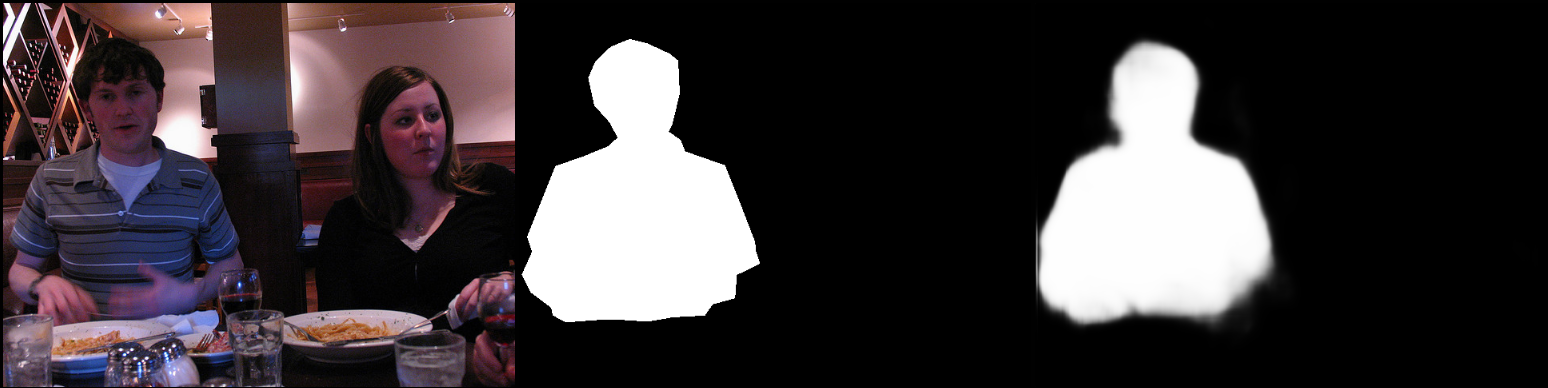
\includegraphics[width=\textwidth]{./figures/unc_samples/1.png}
    \subcaption{Man on left}
    % \label{subfig:original_img}
    \end{subfigure}
    
    \begin{subfigure}[b]{\columnwidth}
            \centering
            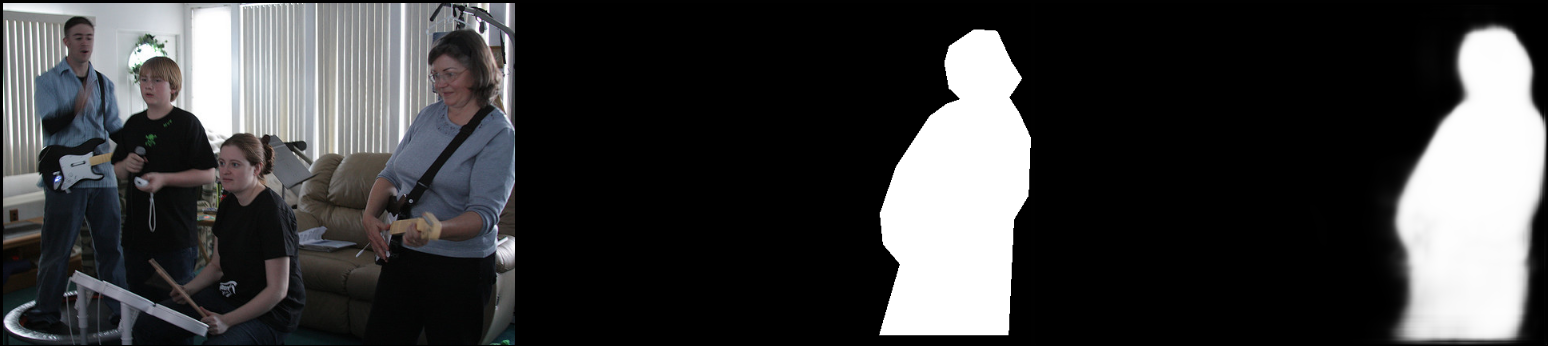
\includegraphics[width=\textwidth]{./figures/unc_samples/2.png}
    \subcaption{Woman on the right}
    % \label{subfig:original_img}
    \end{subfigure}
    
    \begin{subfigure}[b]{\columnwidth}
            \centering
            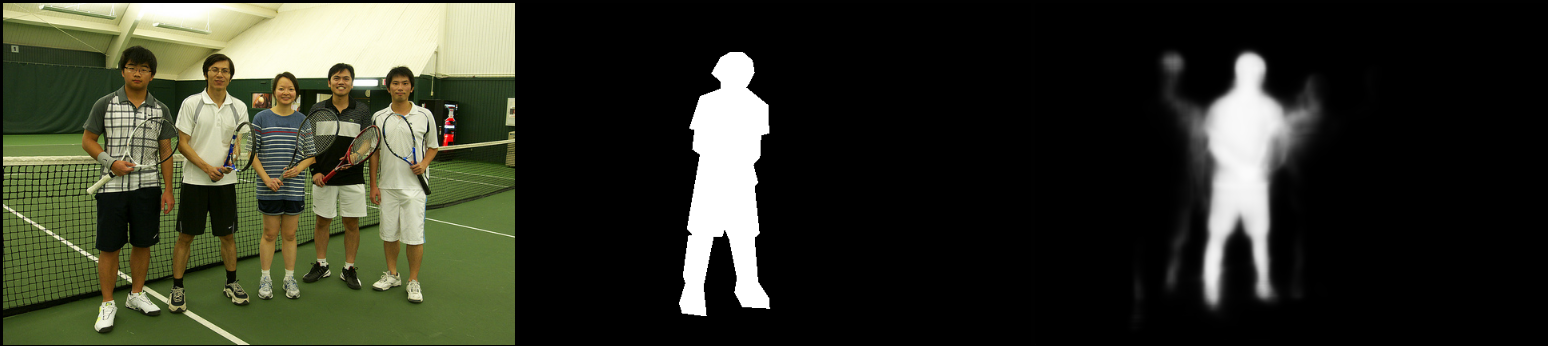
\includegraphics[width=\textwidth]{./figures/unc_samples/3.png}
    \subcaption{Man second from the left with white shirt}
    % \label{subfig:original_img}
    \end{subfigure}
    
    \begin{subfigure}[b]{\columnwidth}
            \centering
            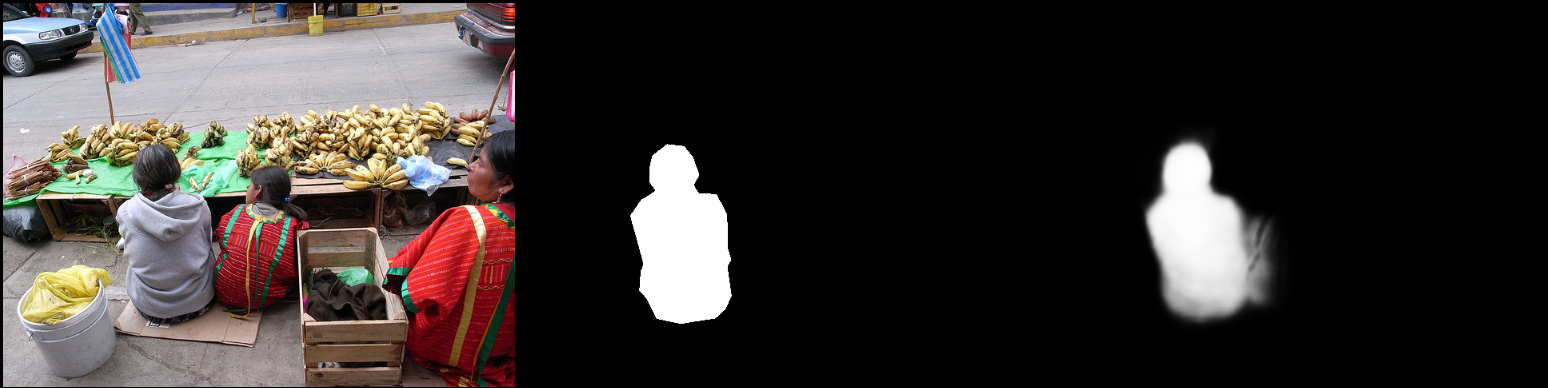
\includegraphics[width=\textwidth]{./figures/unc_samples/4.png}
    \subcaption{Girl sitting on left with gray hoodie}
    % \label{subfig:original_img}
    \end{subfigure}
    \caption{Some DMN positive samples on UNC. \textbf{Left-Right:} Original Image, Reference Mask GT and DMN output mask}
    \label{Fig:UNC_Pos}
\end{figure}
\begin{figure}[!htbp]
    \ContinuedFloat
	\centering
    \begin{subfigure}[b]{\columnwidth}
            \centering
            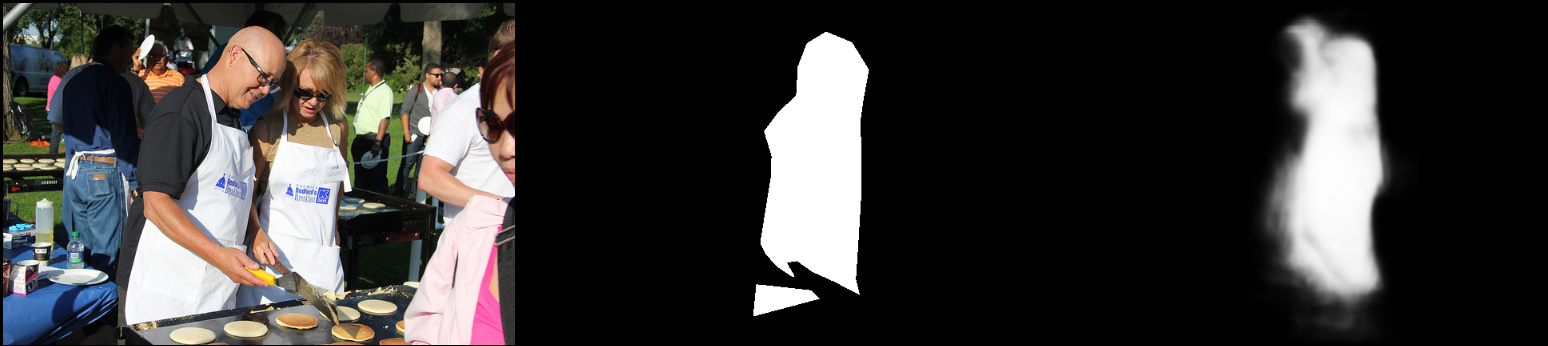
\includegraphics[width=\textwidth]{./figures/unc_samples/5.png}
    \subcaption{Woman with apron}
    % \label{subfig:original_img}
    \end{subfigure}
    \begin{subfigure}[b]{\columnwidth}
            \centering
            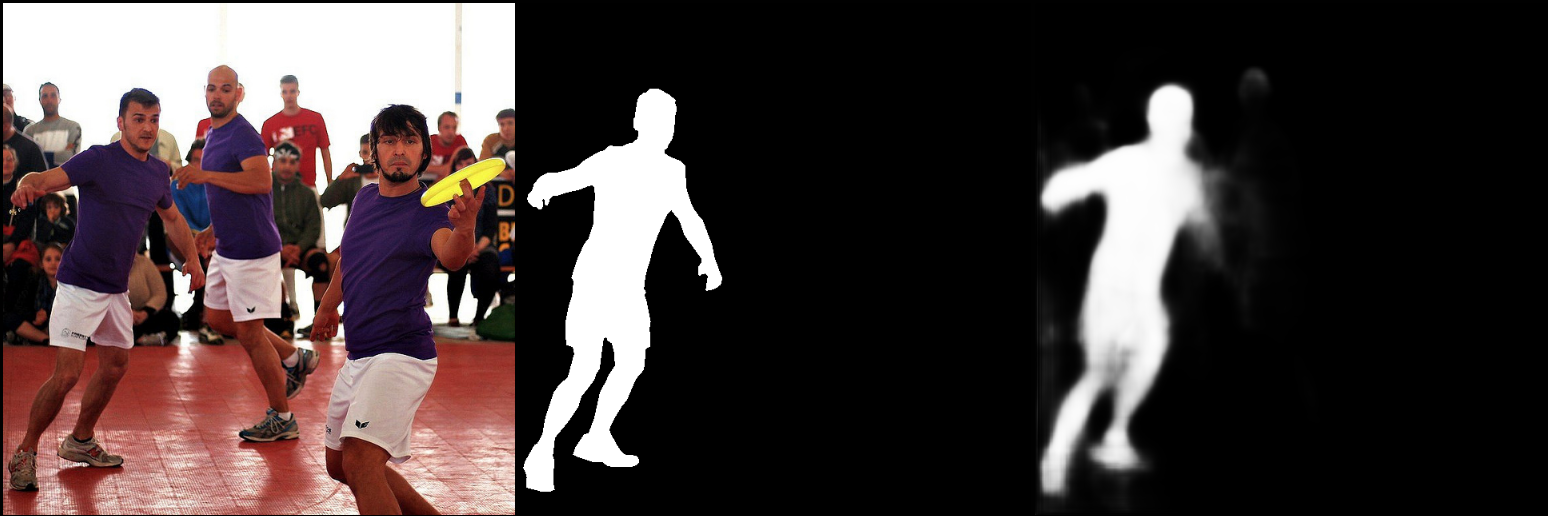
\includegraphics[width=\textwidth]{./figures/unc_samples/6.png}
    \subcaption{Purple shirt on left}
    % \label{subfig:original_img}
    \end{subfigure}
    
    % \begin{subfigure}[b]{0.27\columnwidth}
    %         \centering
    %         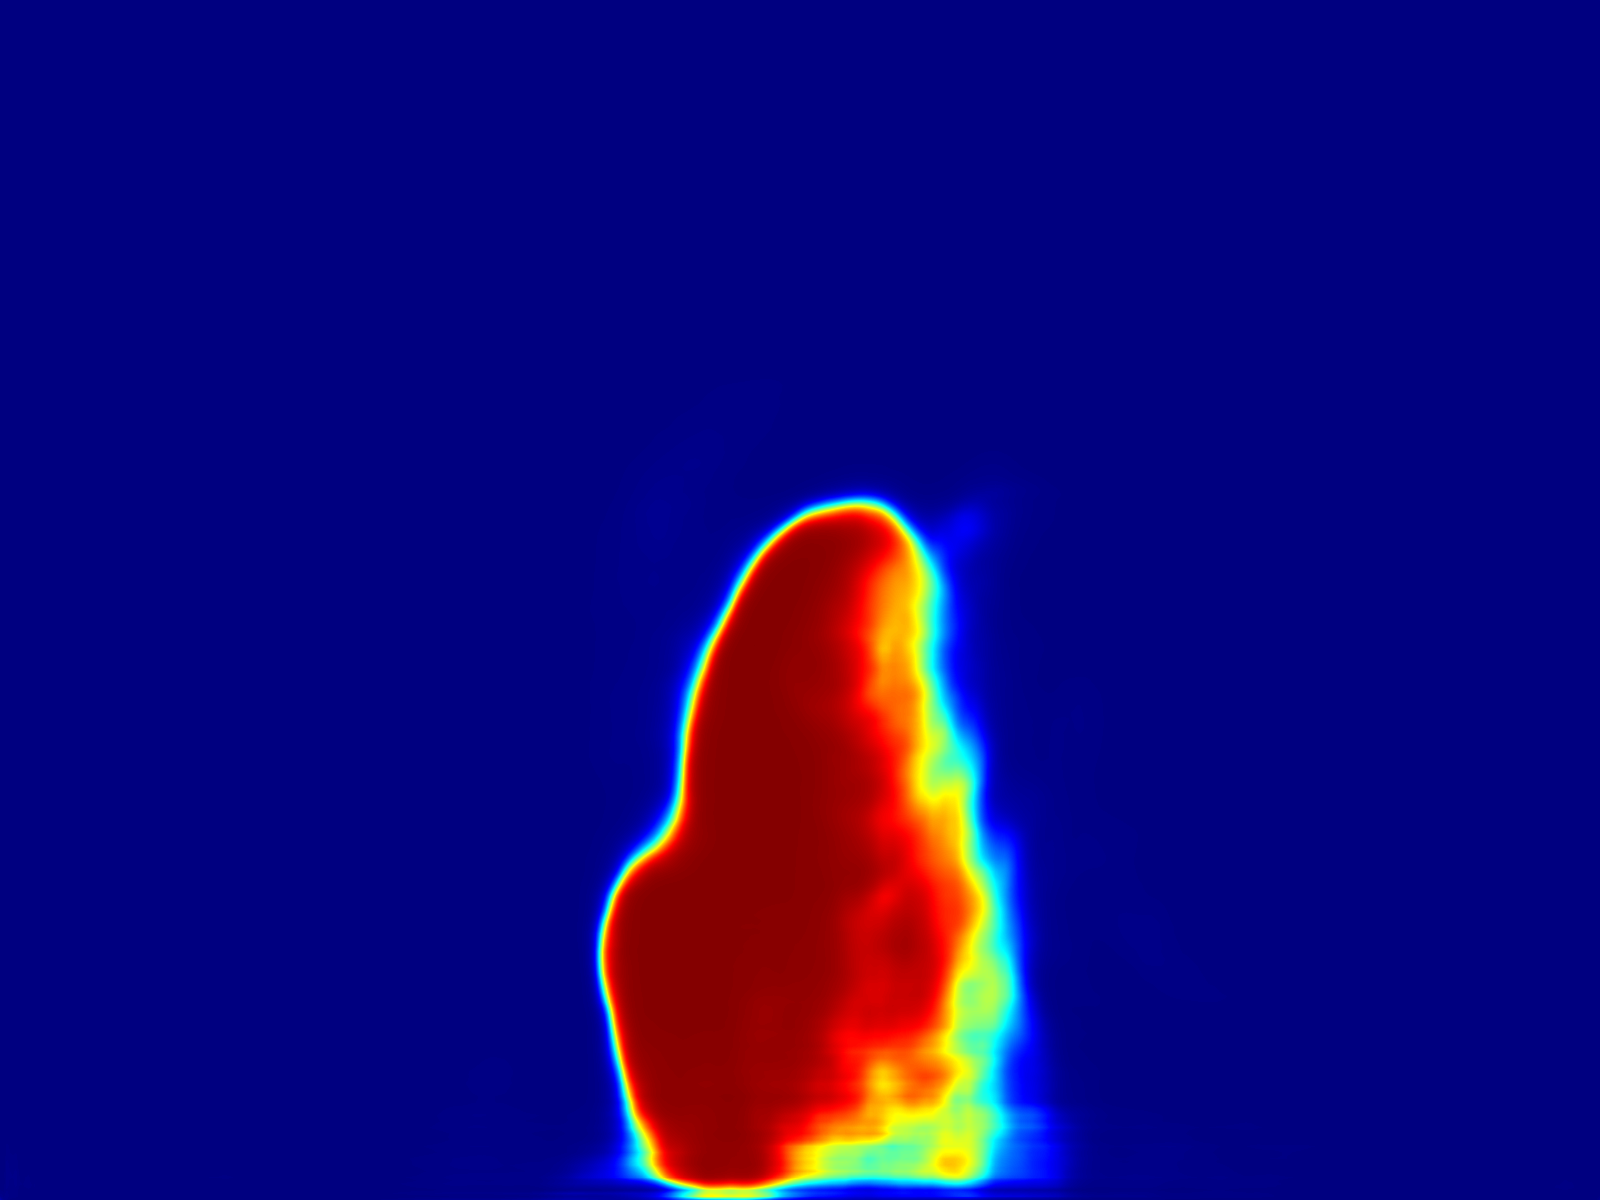
\includegraphics[width=\textwidth]{./figures/Mask_1.png}
    % \subcaption{\textit{Woman on the left}}
    % \label{subfig:woman_left}
    % \end{subfigure}
    %  \begin{subfigure}[b]{0.27\columnwidth}
    %         \centering
    %         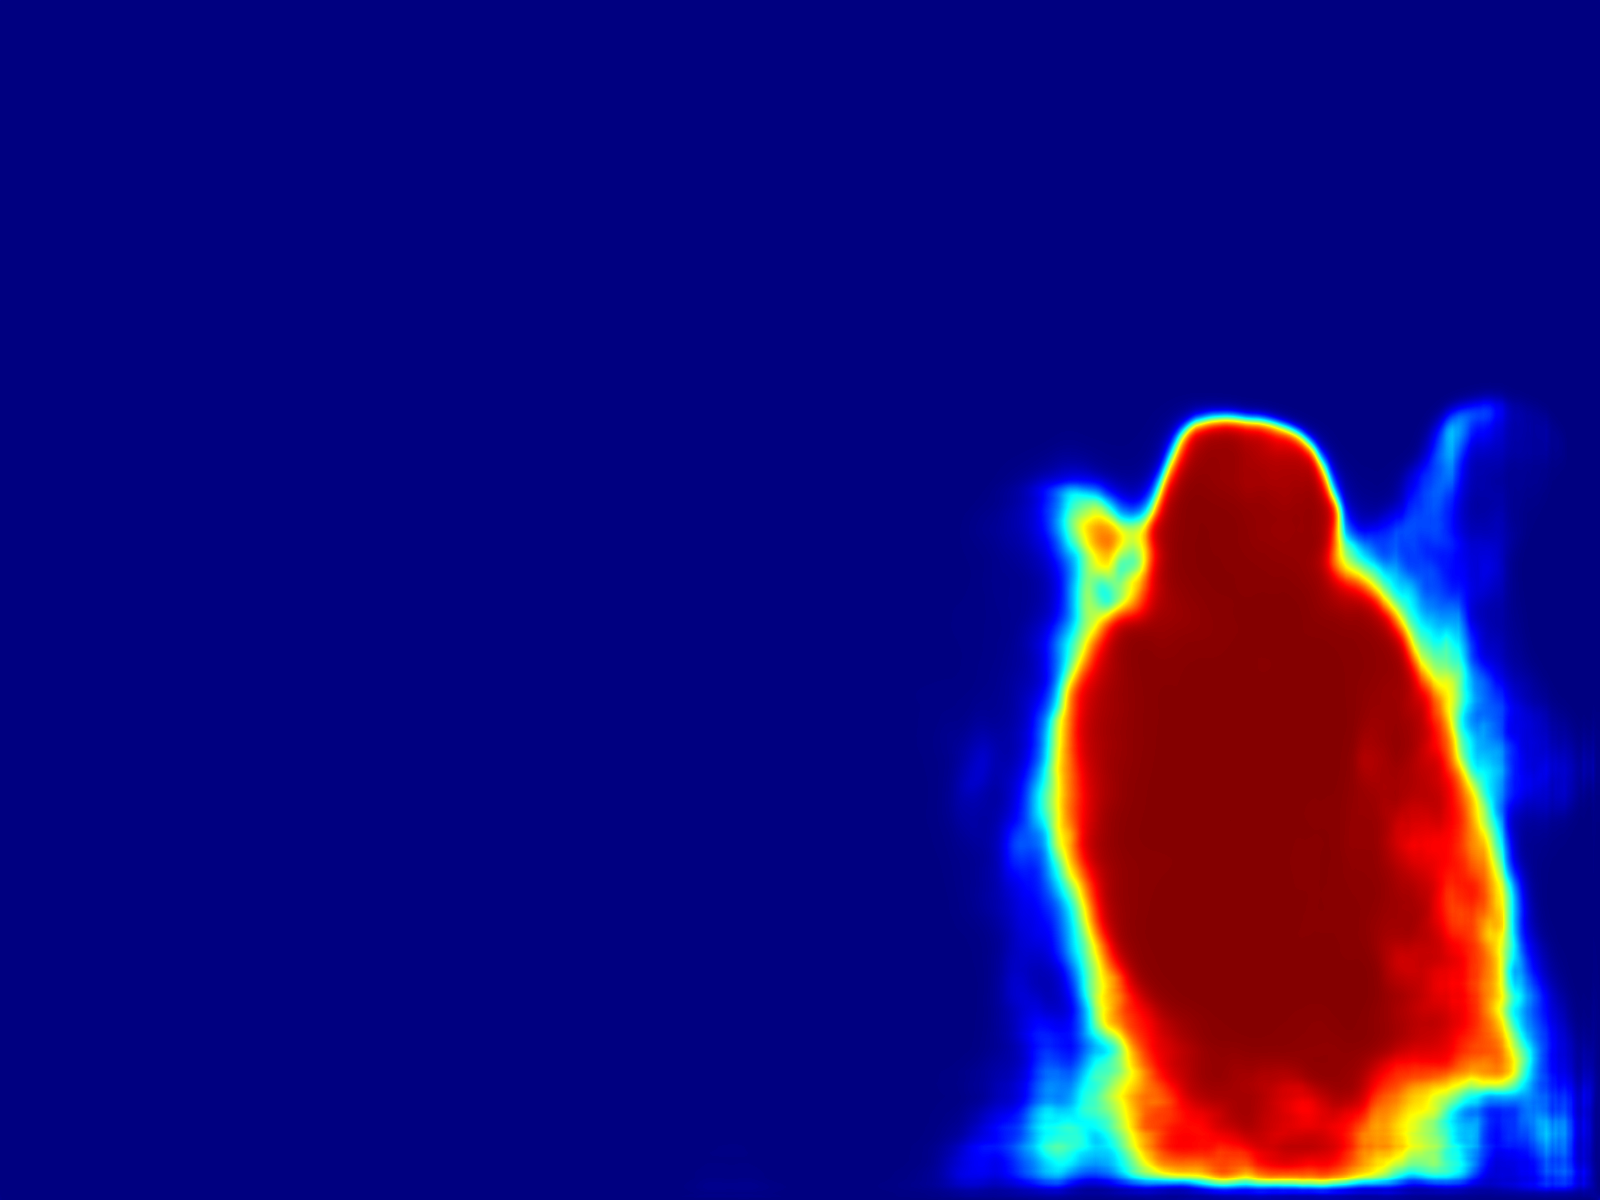
\includegraphics[width=\textwidth]{./figures/Mask_2.png}
    % \subcaption{\textit{Man on blue}}
    % \label{subfig:man_blue}
    % \end{subfigure}
    %\subfloat[Original image.]{{\includegraphics[width=0.25\columnwidth]{./figures/first-fig-1.png} }}%
    %\quad
    %\subfloat[Heatmap based on query \textit{guy}.]{{\includegraphics[width=0.25\columnwidth]{./figures/first-fig-3.png} }}%
    %\quad
    %\subfloat[Heatmap based on query \textit{girl}.]{{\includegraphics[width=0.25\columnwidth]{./figures/girl.png} }}%
    \caption{Some DMN positive samples on UNC. \textbf{Left-Right:} Original Image, Reference Mask GT and DMN output mask}
    \label{Fig:UNC_Pos}
\end{figure}

\begin{figure}[!htbp]
    \centering
    \begin{subfigure}[b]{\columnwidth}
            \centering
            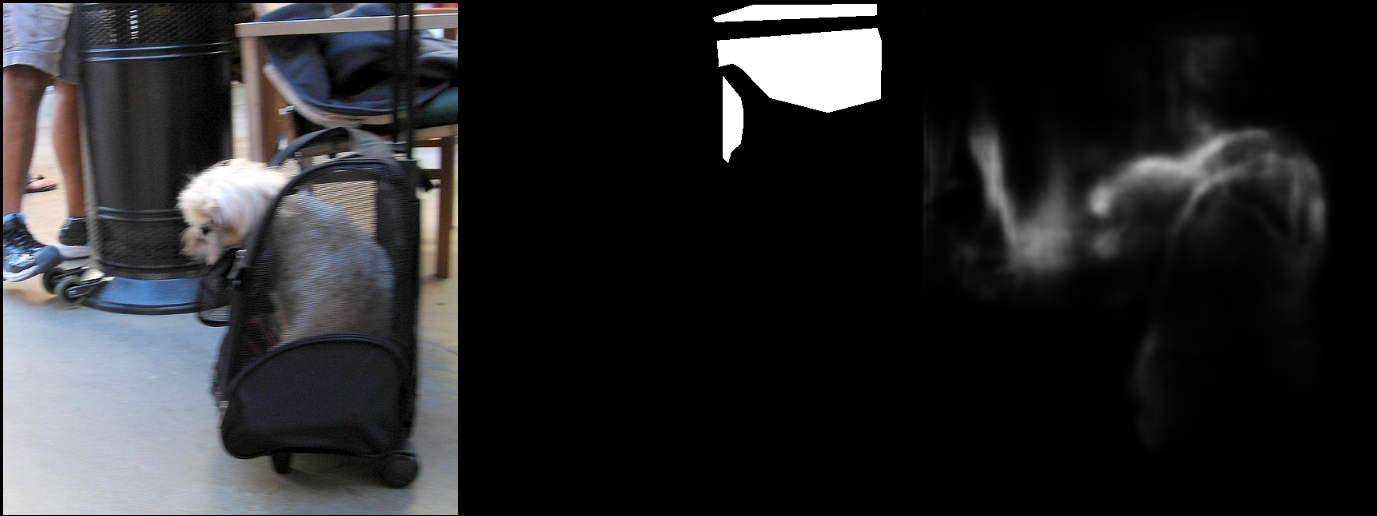
\includegraphics[width=\textwidth]{./figures/unc_samples/1_neg.png}
    \subcaption{Bag in}
    % \label{subfig:original_img}
    \end{subfigure}
    
    \begin{subfigure}[b]{\columnwidth}
            \centering
            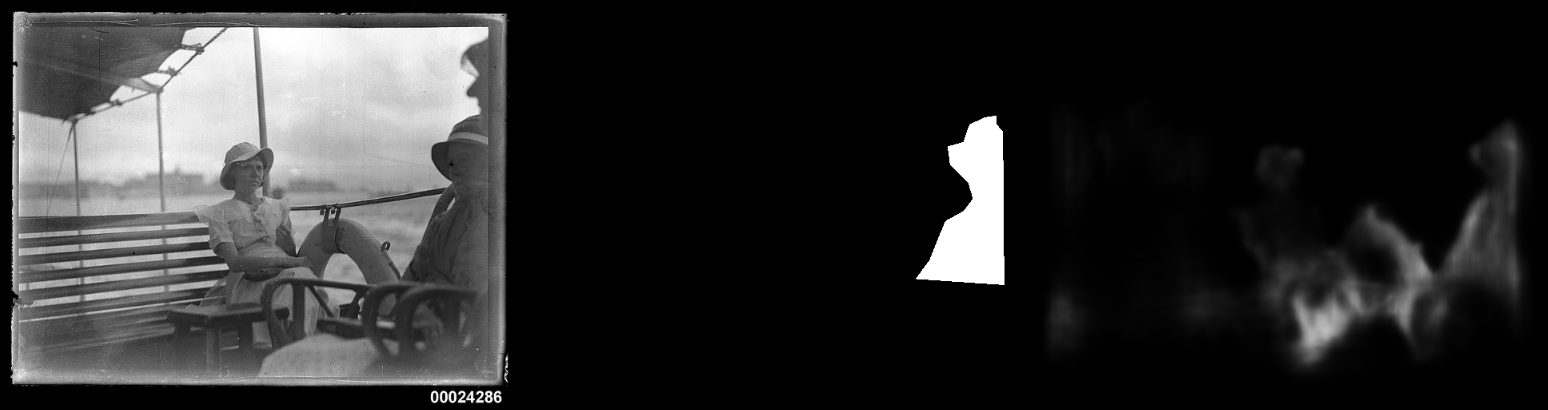
\includegraphics[width=\textwidth]{./figures/unc_samples/2_neg.png}
    \subcaption{Person sitting on the right with a hat that has a white stripe}
    % \label{subfig:original_img}
    \end{subfigure}
    
    \begin{subfigure}[b]{\columnwidth}
            \centering
            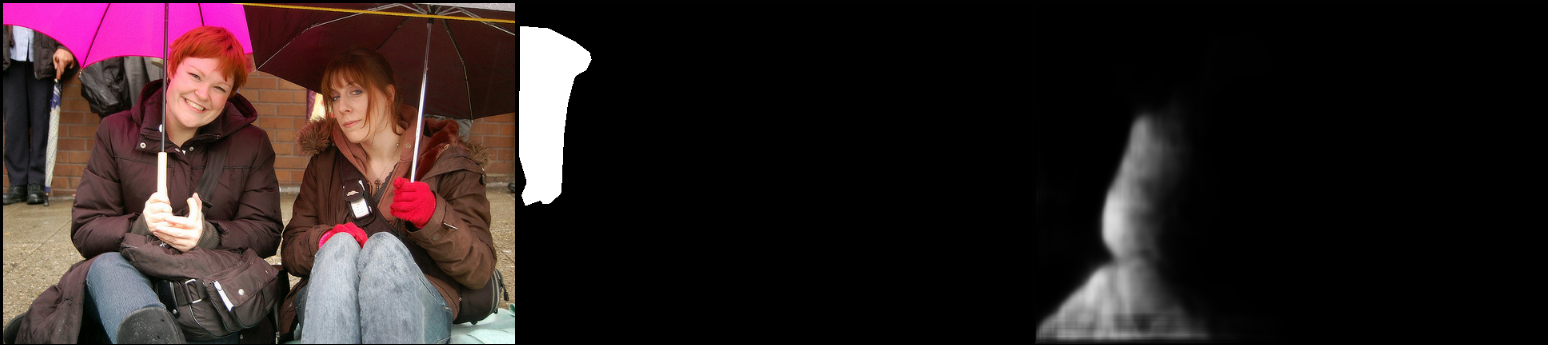
\includegraphics[width=\textwidth]{./figures/unc_samples/3_neg.png}
    \subcaption{Half body far left}
    % \label{subfig:original_img}
    \end{subfigure}
    
    \begin{subfigure}[b]{\columnwidth}
            \centering
            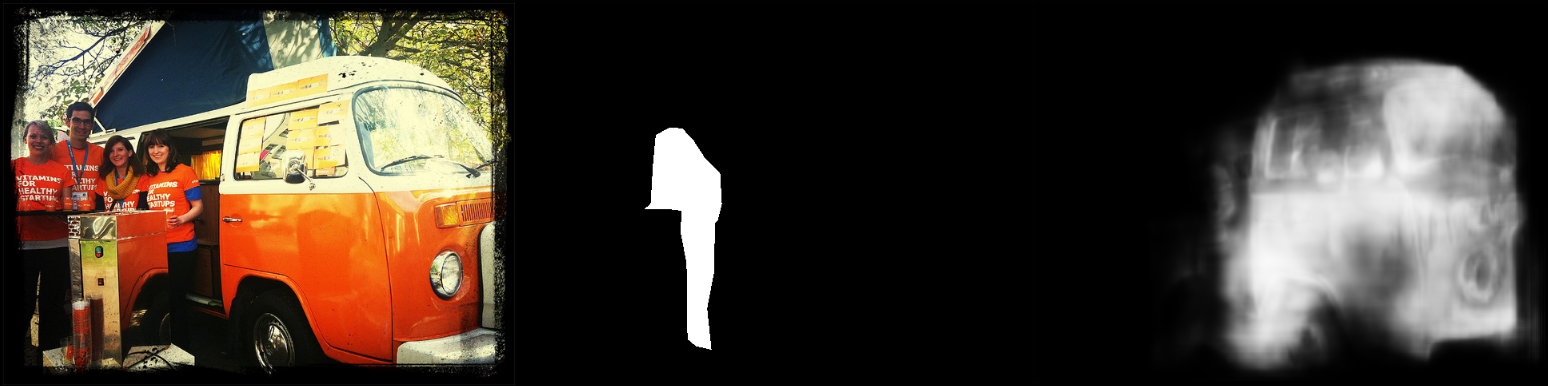
\includegraphics[width=\textwidth]{./figures/unc_samples/4_neg.png}
    \subcaption{Woman on right}
    % \label{subfig:original_img}
    \end{subfigure}
    \caption{Some DMN negative samples on UNC. \textbf{Left-Right:} Original Image, Reference Mask GT and DMN output mask}
    \label{Fig:UNC_Neg}
\end{figure}
\FloatBarrier
\subsection*{UNC+}
\begin{figure}[!htbp]
    \centering
    \begin{subfigure}[b]{\columnwidth}
            \centering
            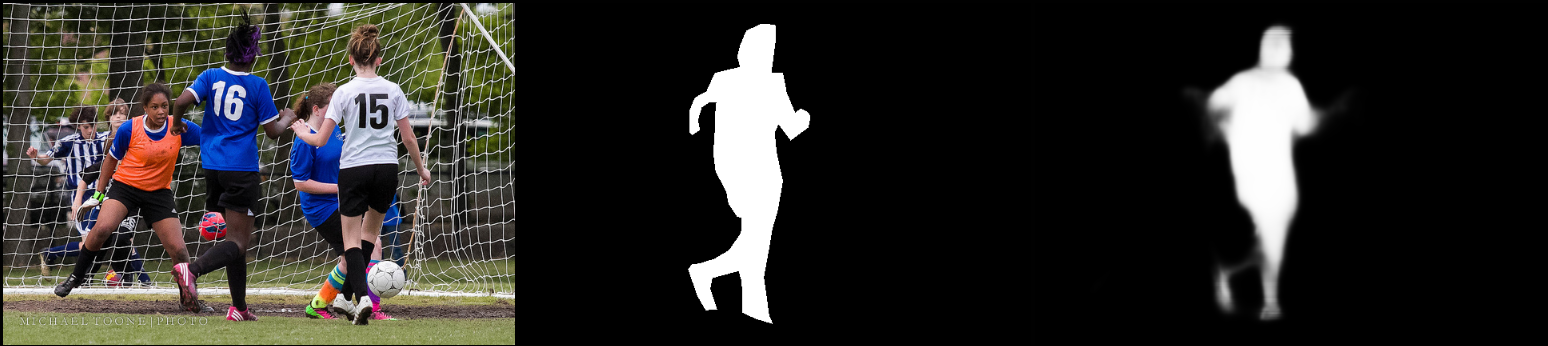
\includegraphics[width=\textwidth]{./figures/unc_plus_samples/5.png}
    \subcaption{Player on shirt 16}
    % \label{subfig:original_img}
    \end{subfigure}
    
    \begin{subfigure}[b]{\columnwidth}
            \centering
            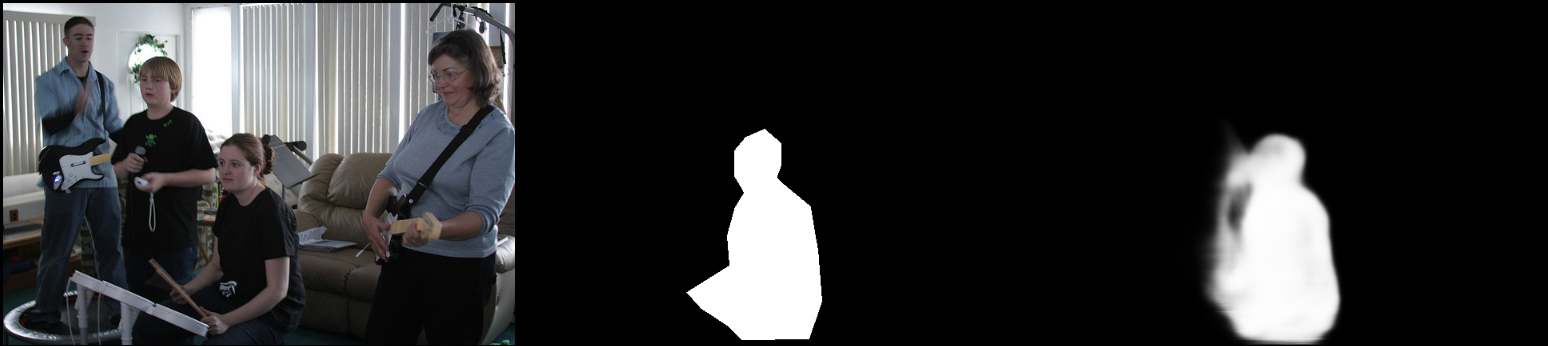
\includegraphics[width=\textwidth]{./figures/unc_plus_samples/6.png}
    \subcaption{Person sitting}
    % \label{subfig:original_img}
    \end{subfigure}
    
    \begin{subfigure}[b]{\columnwidth}
            \centering
            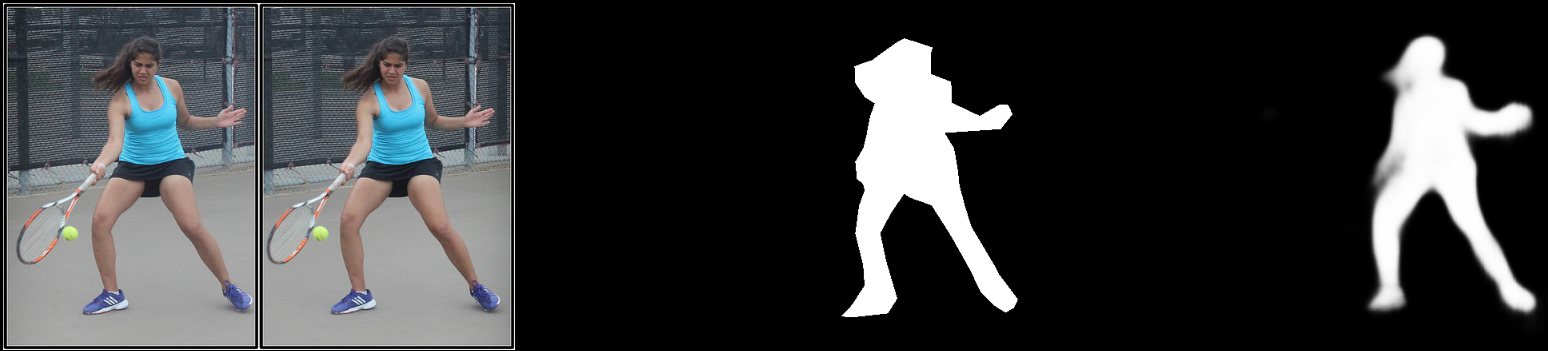
\includegraphics[width=\textwidth]{./figures/unc_plus_samples/3.png}
    \subcaption{Girl in picture 2}
    % \label{subfig:original_img}
    \end{subfigure}
    
    \begin{subfigure}[b]{\columnwidth}
            \centering
            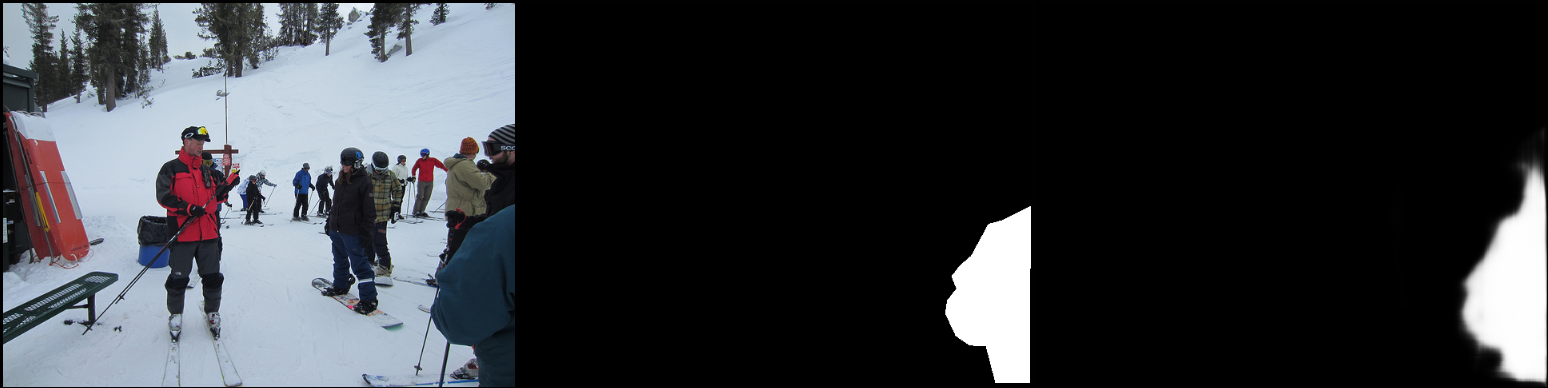
\includegraphics[width=\textwidth]{./figures/unc_plus_samples/4.png}
    \subcaption{Blue jacket partial}
    % \label{subfig:original_img}
    \end{subfigure}
    \caption{Some DMN positive samples on UNC+. \textbf{Left-Right:} Original Image, Reference Mask GT and DMN output mask}
    \label{Fig:UNC+_Pos}
\end{figure}
\begin{figure}[!htbp]
    \ContinuedFloat
	\centering
    \begin{subfigure}[b]{\columnwidth}
            \centering
            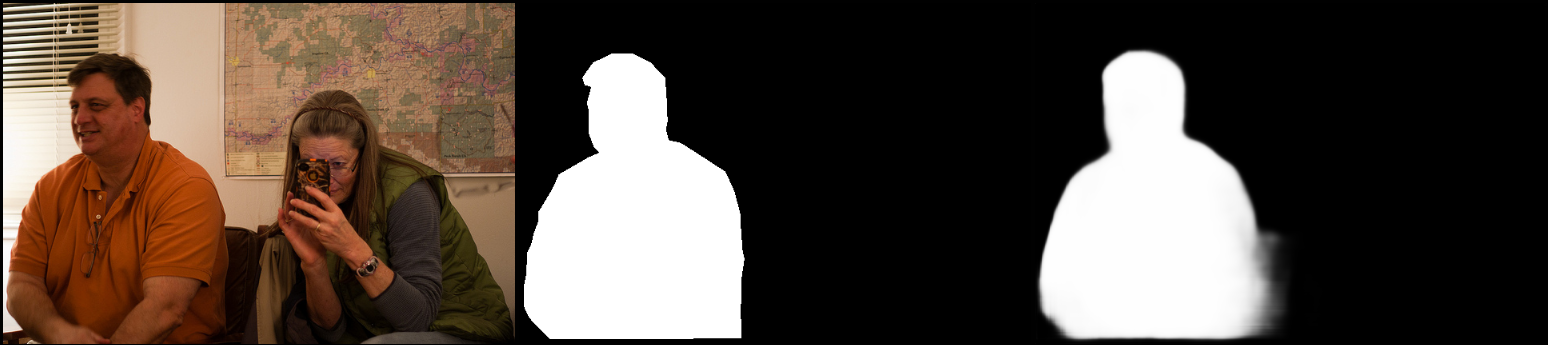
\includegraphics[width=\textwidth]{./figures/unc_plus_samples/1.png}
    \subcaption{Man in orange shirt}
    % \label{subfig:original_img}
    \end{subfigure}
    \begin{subfigure}[b]{\columnwidth}
            \centering
            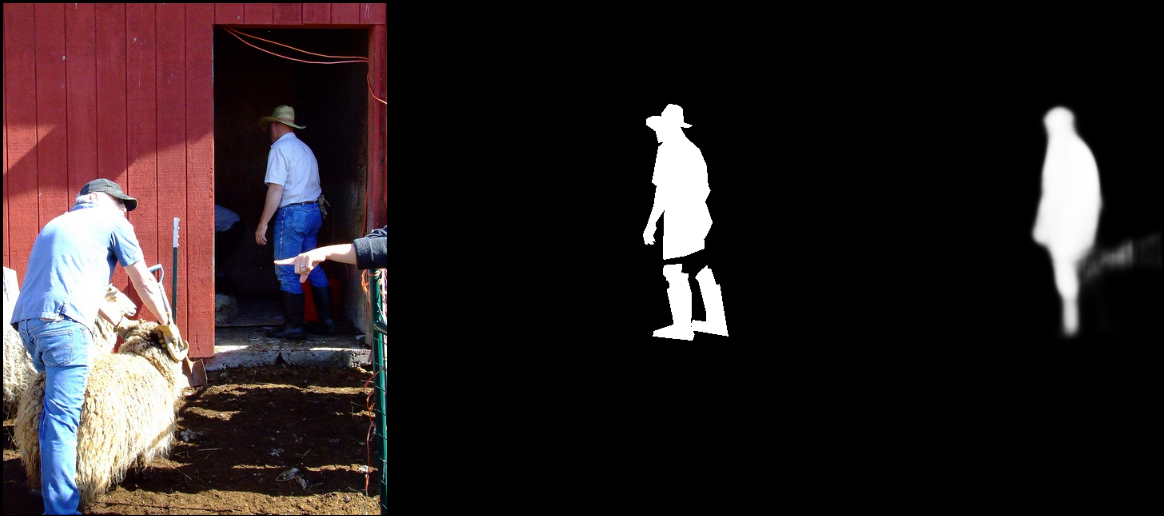
\includegraphics[width=\textwidth]{./figures/unc_plus_samples/2.png}
    \subcaption{Man in doorway}
    % \label{subfig:original_img}
    \end{subfigure}
    
    % \begin{subfigure}[b]{0.27\columnwidth}
    %         \centering
    %         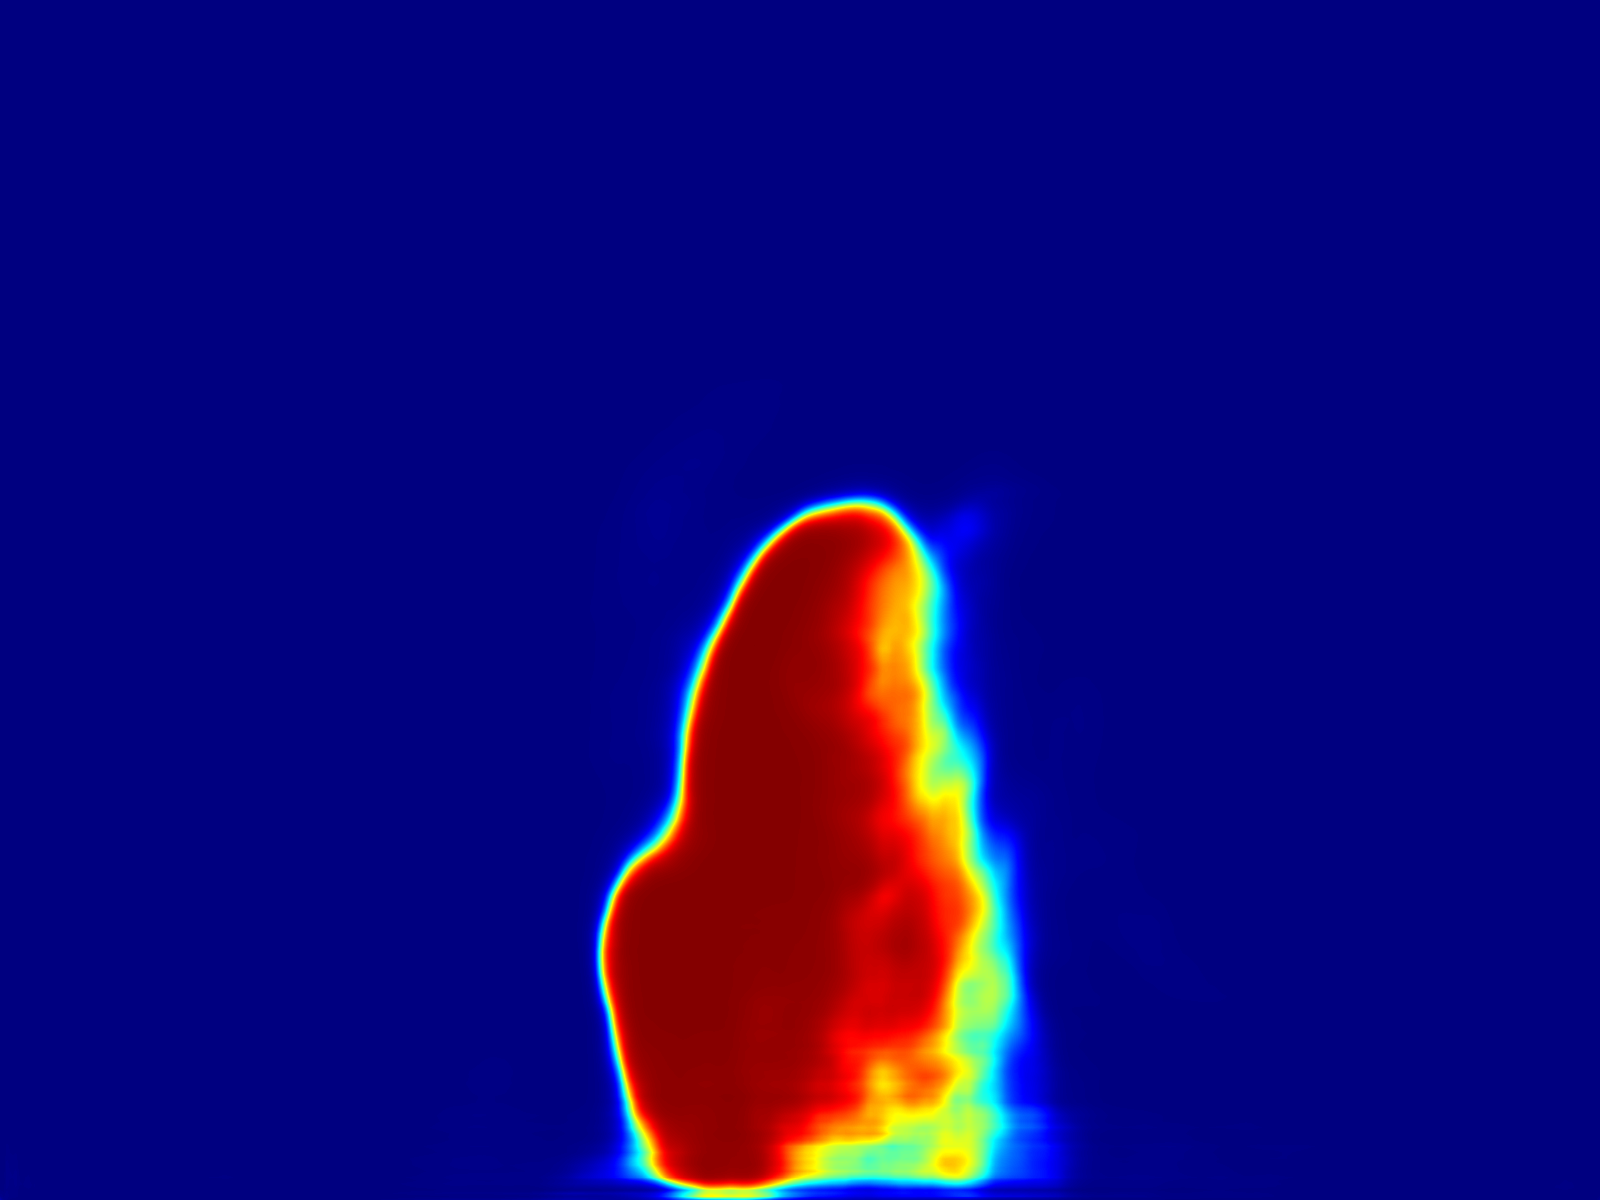
\includegraphics[width=\textwidth]{./figures/Mask_1.png}
    % \subcaption{\textit{Woman on the left}}
    % \label{subfig:woman_left}
    % \end{subfigure}
    %  \begin{subfigure}[b]{0.27\columnwidth}
    %         \centering
    %         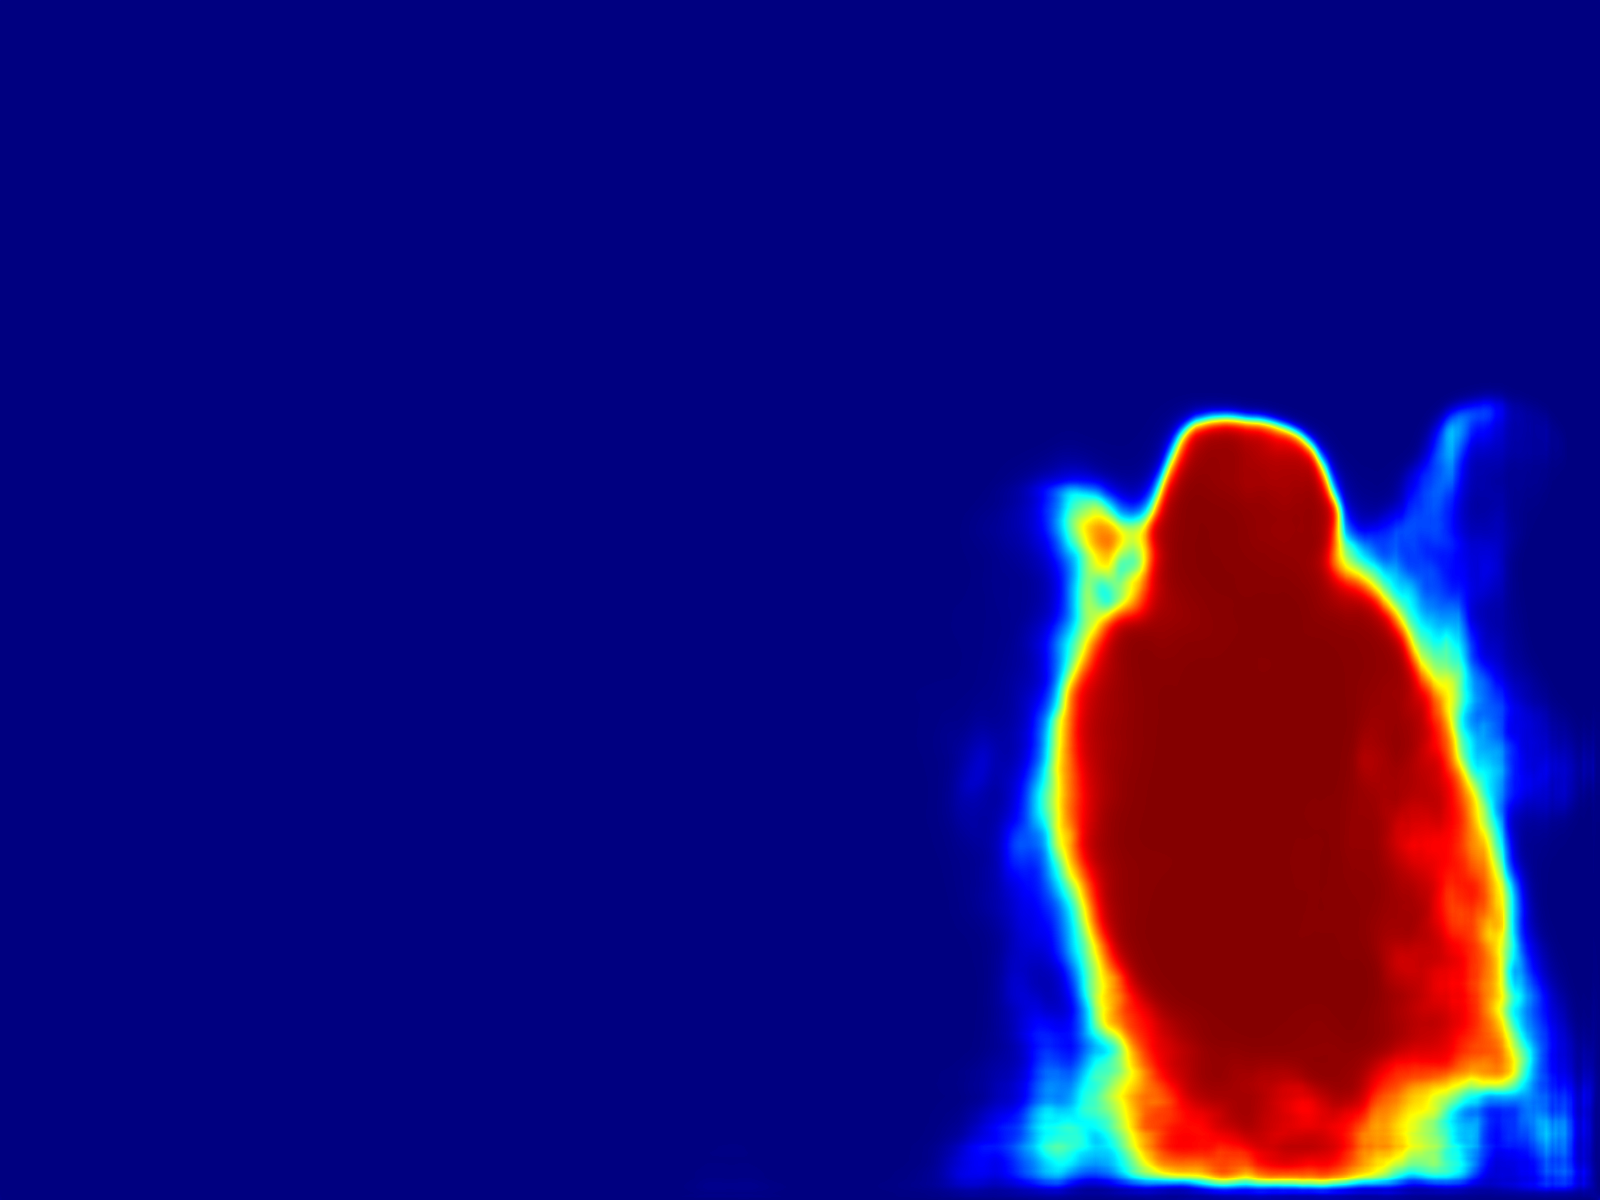
\includegraphics[width=\textwidth]{./figures/Mask_2.png}
    % \subcaption{\textit{Man on blue}}
    % \label{subfig:man_blue}
    % \end{subfigure}
    %\subfloat[Original image.]{{\includegraphics[width=0.25\columnwidth]{./figures/first-fig-1.png} }}%
    %\quad
    %\subfloat[Heatmap based on query \textit{guy}.]{{\includegraphics[width=0.25\columnwidth]{./figures/first-fig-3.png} }}%
    %\quad
    %\subfloat[Heatmap based on query \textit{girl}.]{{\includegraphics[width=0.25\columnwidth]{./figures/girl.png} }}%
    \caption{Some DMN positive samples on UNC+. \textbf{Left-Right:} Original Image, Reference Mask GT and DMN output mask}
    \label{Fig:UNC+_Pos}
\end{figure}

\begin{figure}[!htbp]
    \centering
    \begin{subfigure}[b]{\columnwidth}
            \centering
            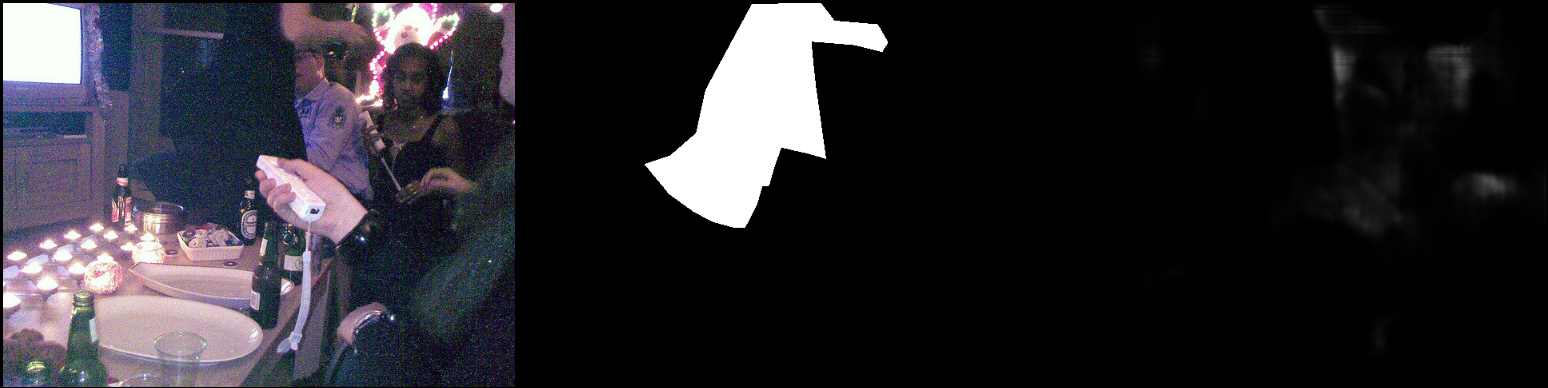
\includegraphics[width=\textwidth]{./figures/unc_plus_samples/1_neg.png}
    \subcaption{Black blur at the end of the remote}
    % \label{subfig:original_img}
    \end{subfigure}
    
    \begin{subfigure}[b]{\columnwidth}
            \centering
            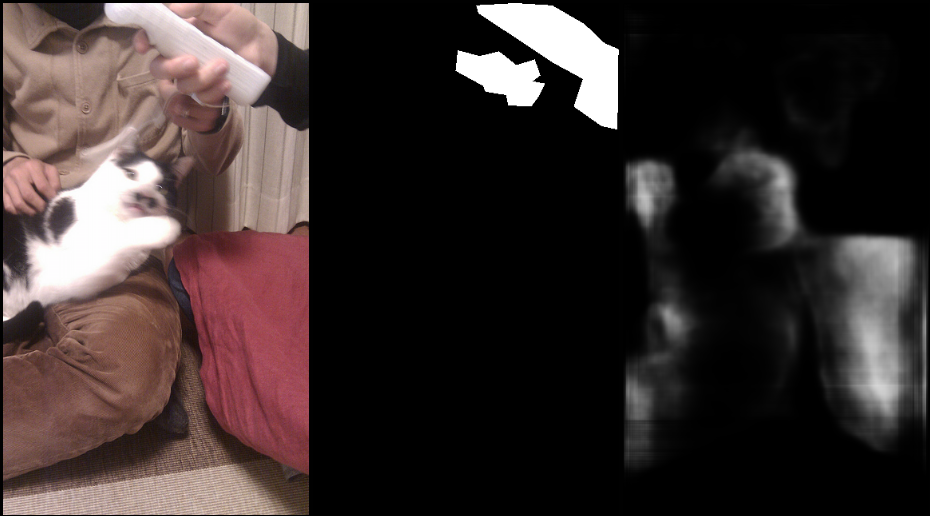
\includegraphics[width=\textwidth]{./figures/unc_plus_samples/2_neg.png}
    \subcaption{The hand holding the white object}
    % \label{subfig:original_img}
    \end{subfigure}
    
    \begin{subfigure}[b]{\columnwidth}
            \centering
            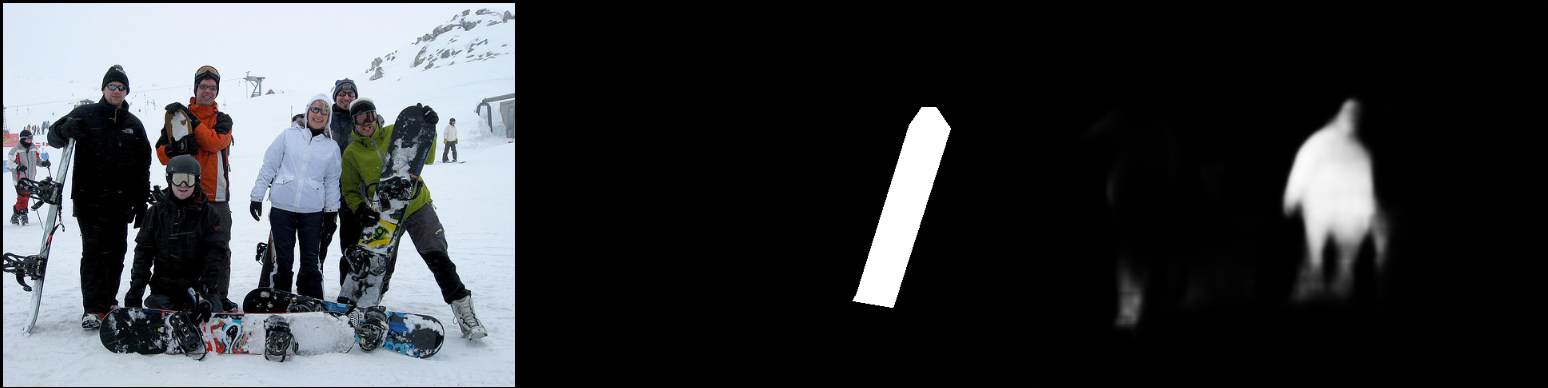
\includegraphics[width=\textwidth]{./figures/unc_plus_samples/3_neg.png}
    \subcaption{Decorated snowboard upright}
    % \label{subfig:original_img}
    \end{subfigure}
    
    \begin{subfigure}[b]{\columnwidth}
            \centering
            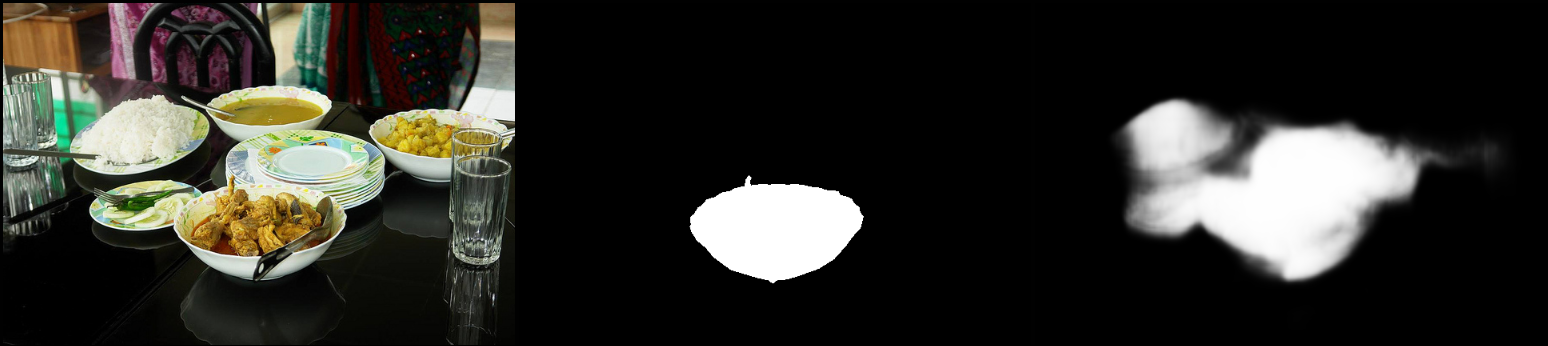
\includegraphics[width=\textwidth]{./figures/unc_plus_samples/4_neg.png}
    \subcaption{Closest bowl}
    % \label{subfig:original_img}
    \end{subfigure}
    \caption{Some DMN negative samples on UNC+. \textbf{Left-Right:} Original Image, Reference Mask GT and DMN output mask}
    \label{Fig:UNC+_Neg}
\end{figure}


\FloatBarrier
\subsection*{GRef}
\begin{figure}[!htbp]
    \centering
    \begin{subfigure}[b]{\columnwidth}
            \centering
            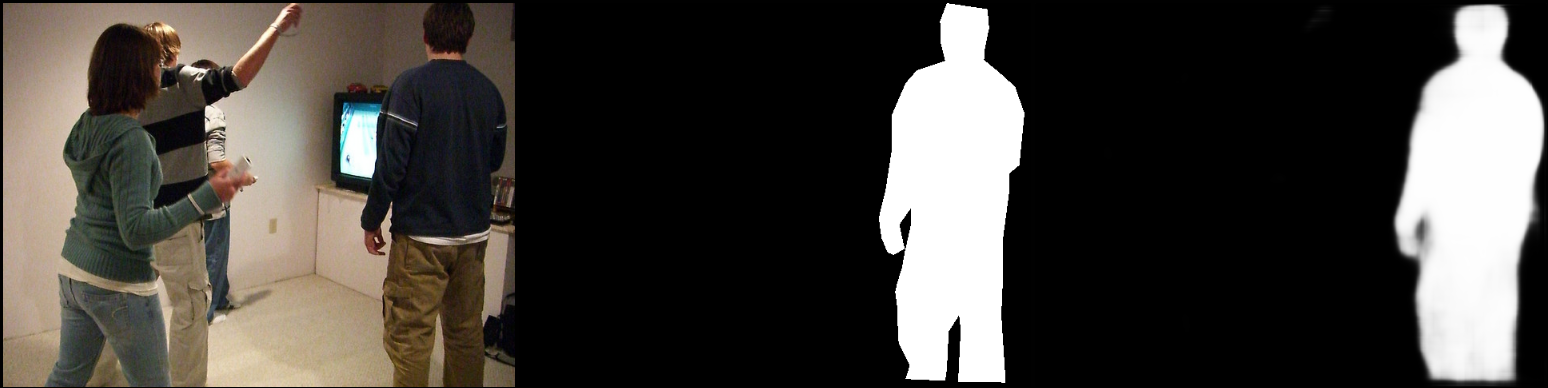
\includegraphics[width=\textwidth]{./figures/gref_samples/1.png}
    \subcaption{A man in a arm striped sweater}
    % \label{subfig:original_img}
    \end{subfigure}
    
    \begin{subfigure}[b]{\columnwidth}
            \centering
            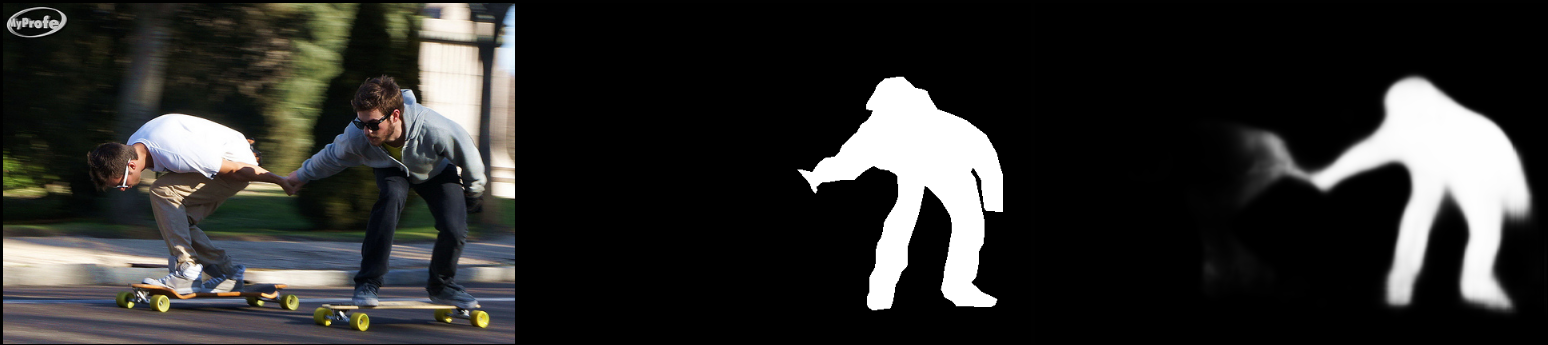
\includegraphics[width=\textwidth]{./figures/gref_samples/2.png}
    \subcaption{A skateboarder with black sunglasses and a grey top}
    % \label{subfig:original_img}
    \end{subfigure}
    
    \begin{subfigure}[b]{\columnwidth}
            \centering
            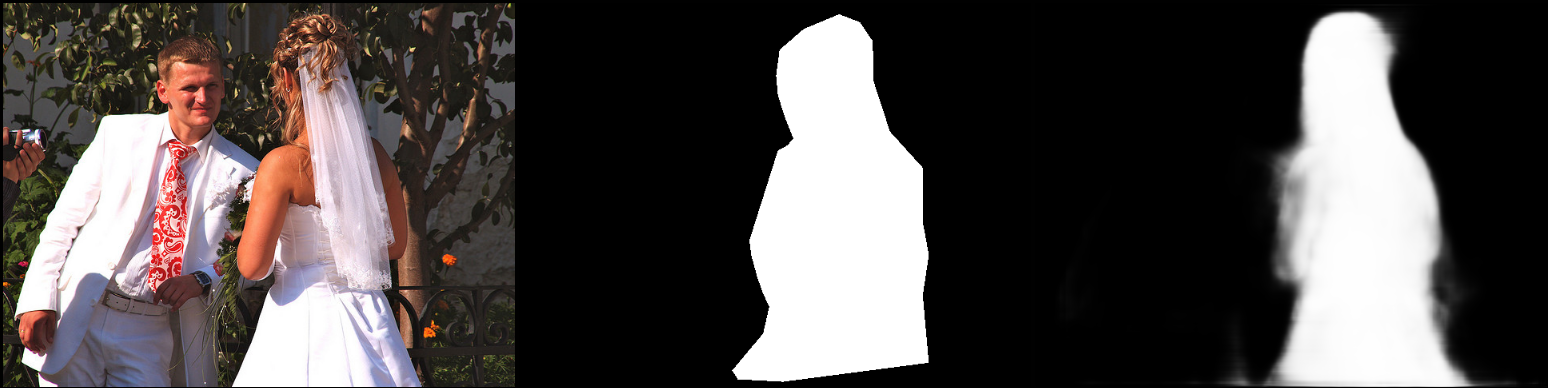
\includegraphics[width=\textwidth]{./figures/gref_samples/3.png}
    \subcaption{The bride wearing a white dress who has light brown hair}
    % \label{subfig:original_img}
    \end{subfigure}
    
    \begin{subfigure}[b]{\columnwidth}
            \centering
            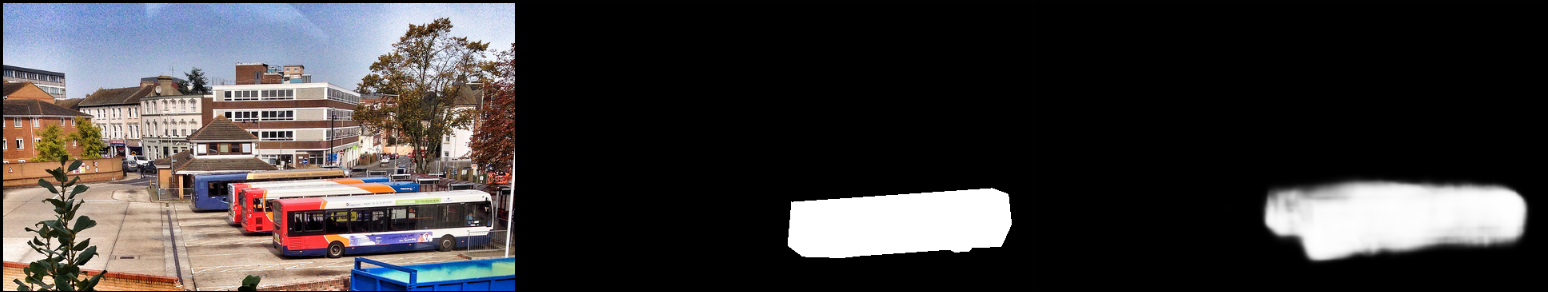
\includegraphics[width=\textwidth]{./figures/gref_samples/5.png}
    \subcaption{A bus in front of others}
    % \label{subfig:original_img}
    \end{subfigure}
    \caption{Some DMN positive samples on GRef. \textbf{Left-Right:} Original Image, Reference Mask GT and DMN output mask}
    \label{Fig:GRef_Pos}
\end{figure}

\begin{figure}[!htbp]
    \ContinuedFloat
	\centering
    
    \begin{subfigure}[b]{\columnwidth}
            \centering
            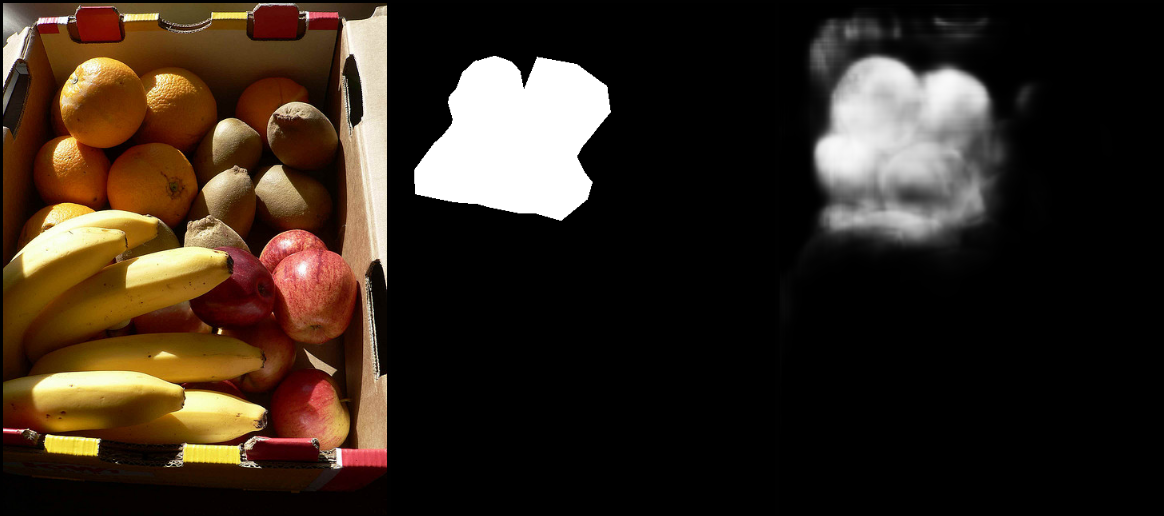
\includegraphics[width=\textwidth]{./figures/gref_samples/4.png}
    \subcaption{The oranges in the basket of fruit}
    % \label{subfig:original_img}
    \end{subfigure}
    \begin{subfigure}[b]{\columnwidth}
            \centering
            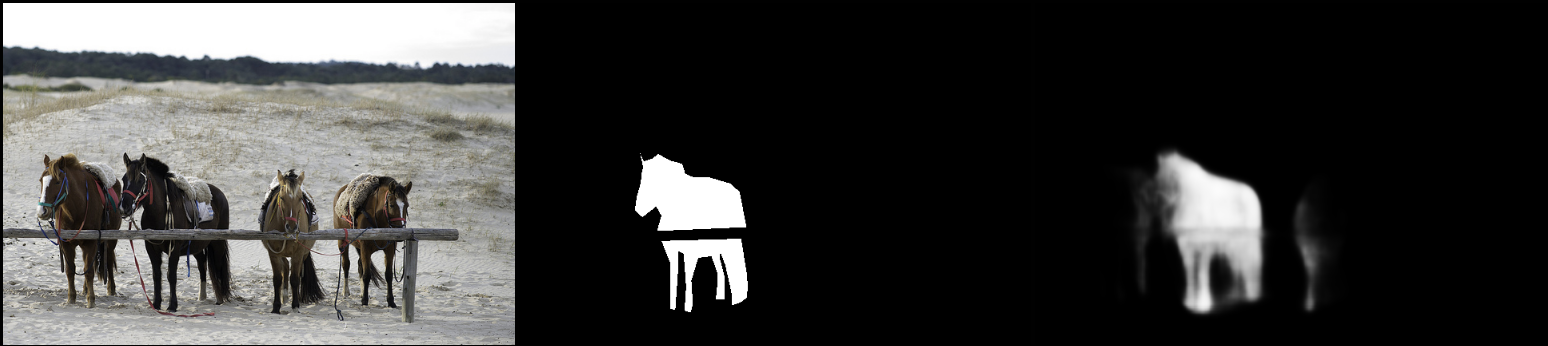
\includegraphics[width=\textwidth]{./figures/gref_samples/6.png}
    \subcaption{A dark horse between three lighter horse}
    % \label{subfig:original_img}
    \end{subfigure}
    
    % \begin{subfigure}[b]{0.27\columnwidth}
    %         \centering
    %         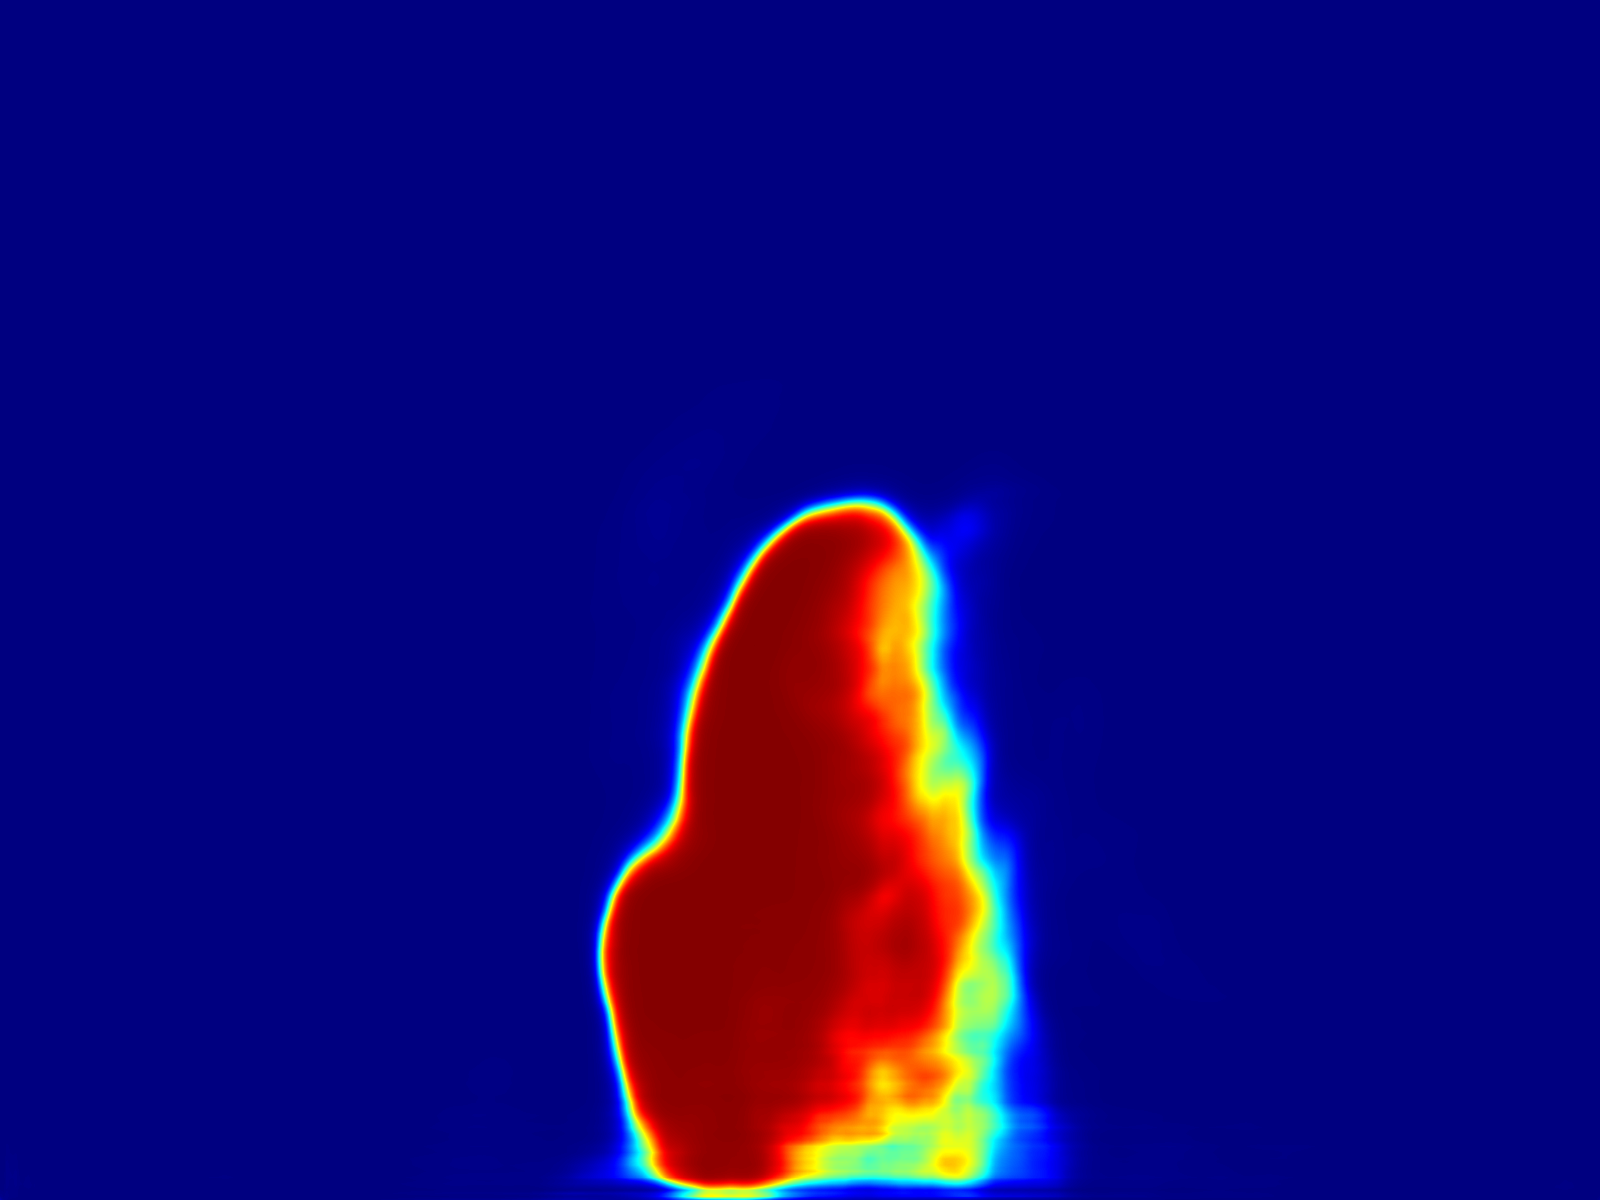
\includegraphics[width=\textwidth]{./figures/Mask_1.png}
    % \subcaption{\textit{Woman on the left}}
    % \label{subfig:woman_left}
    % \end{subfigure}
    %  \begin{subfigure}[b]{0.27\columnwidth}
    %         \centering
    %         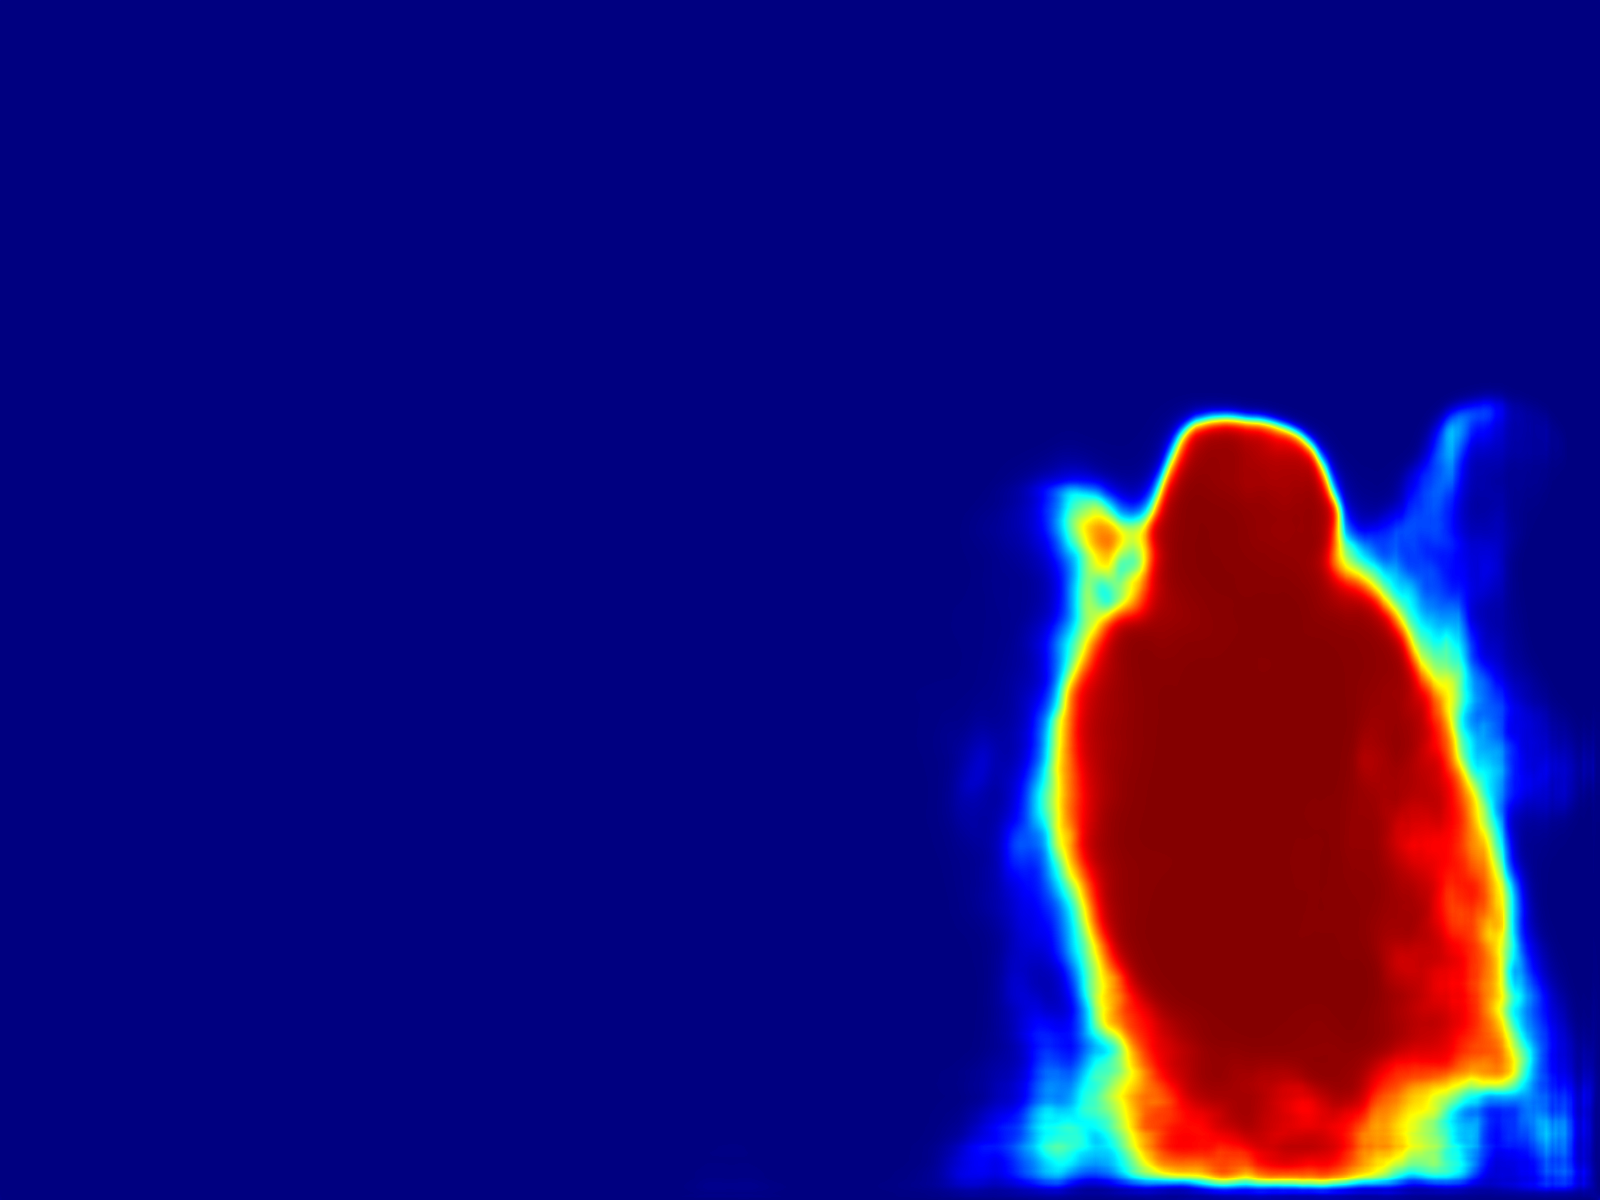
\includegraphics[width=\textwidth]{./figures/Mask_2.png}
    % \subcaption{\textit{Man on blue}}
    % \label{subfig:man_blue}
    % \end{subfigure}
    %\subfloat[Original image.]{{\includegraphics[width=0.25\columnwidth]{./figures/first-fig-1.png} }}%
    %\quad
    %\subfloat[Heatmap based on query \textit{guy}.]{{\includegraphics[width=0.25\columnwidth]{./figures/first-fig-3.png} }}%
    %\quad
    %\subfloat[Heatmap based on query \textit{girl}.]{{\includegraphics[width=0.25\columnwidth]{./figures/girl.png} }}%
    \caption{Some DMN positive samples on GRef. \textbf{Left-Right:} Original Image, Reference Mask GT and DMN output mask}
    \label{Fig:GRef_Pos}
\end{figure}

\begin{figure}[!htbp]
    \centering
    \begin{subfigure}[b]{\columnwidth}
            \centering
            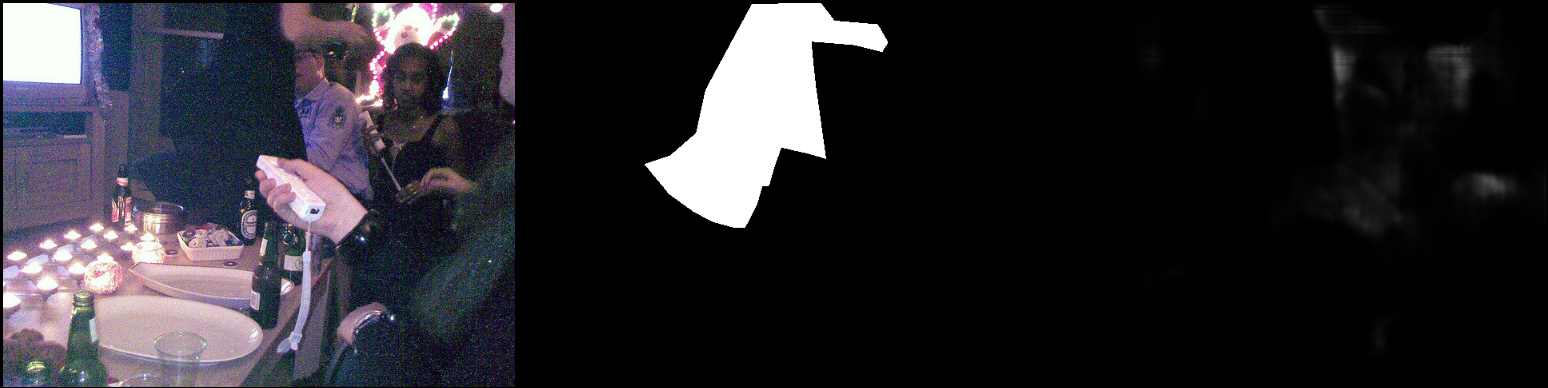
\includegraphics[width=\textwidth]{./figures/unc_plus_samples/1_neg.png}
    \subcaption{Black blur at the end of the remote}
    % \label{subfig:original_img}
    \end{subfigure}
    
    \begin{subfigure}[b]{\columnwidth}
            \centering
            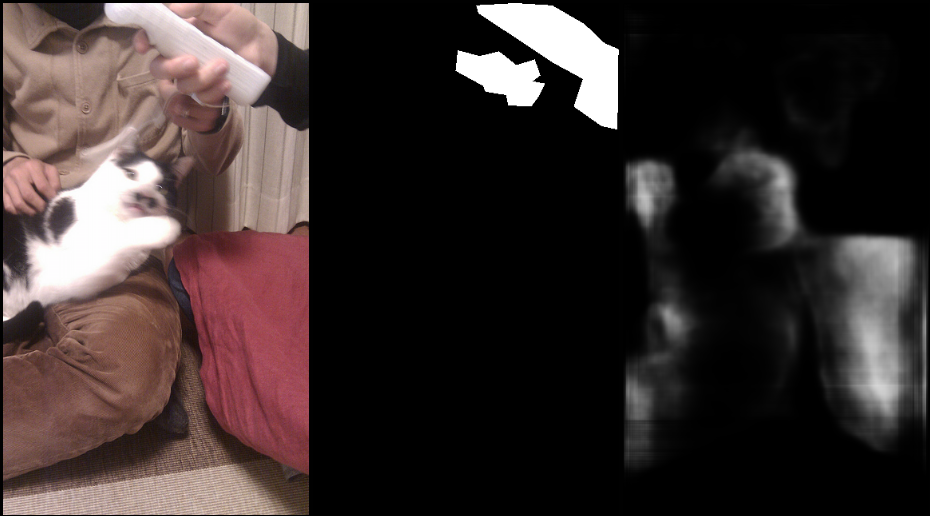
\includegraphics[width=\textwidth]{./figures/unc_plus_samples/2_neg.png}
    \subcaption{The hand holding the white object}
    % \label{subfig:original_img}
    \end{subfigure}
    
    \begin{subfigure}[b]{\columnwidth}
            \centering
            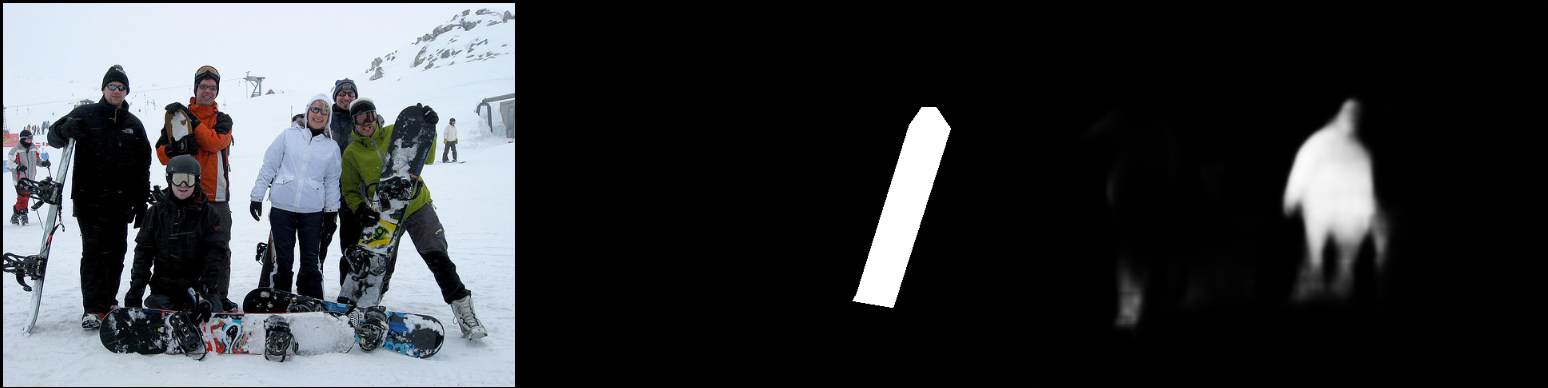
\includegraphics[width=\textwidth]{./figures/unc_plus_samples/3_neg.png}
    \subcaption{Decorated snowboard upright}
    % \label{subfig:original_img}
    \end{subfigure}
    
    \begin{subfigure}[b]{\columnwidth}
            \centering
            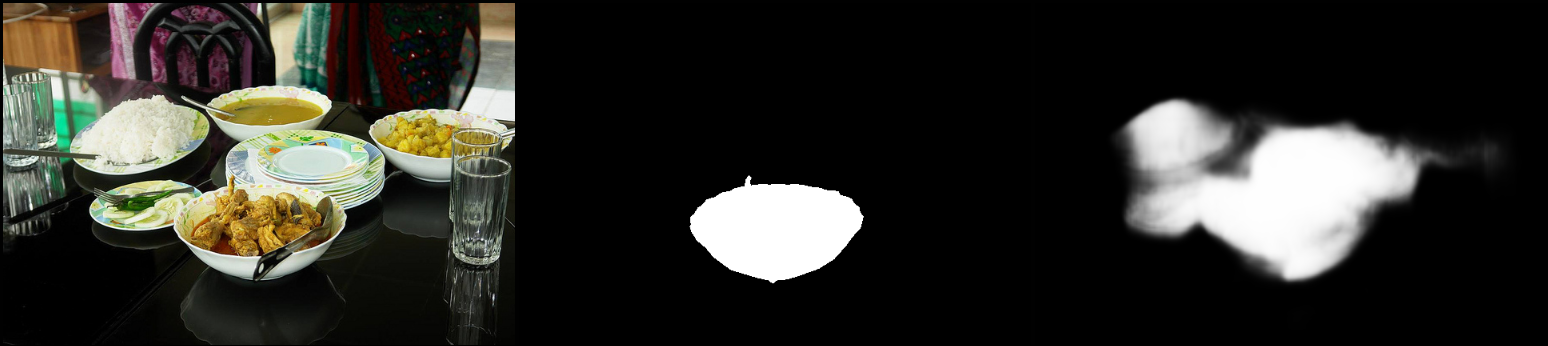
\includegraphics[width=\textwidth]{./figures/unc_plus_samples/4_neg.png}
    \subcaption{Closest bowl}
    % \label{subfig:original_img}
    \end{subfigure}
    \caption{Some DMN negative samples on GRef. \textbf{Left-Right:} Original Image, Reference Mask GT and DMN output mask}
    \label{Fig:GRef_Neg}
\end{figure}
\FloatBarrier
\subsection*{ReferIt}

\section{Additional Experiments}